\documentclass[10pt]{book}
\usepackage{graphicx}
\usepackage{graphics}
\usepackage{subcaption} % Para subfiguras
\usepackage{wrapfig}
\usepackage[hidelinks]{hyperref} %con 
\usepackage[spanish]{babel}
\usepackage{float}
\usepackage{minted}
\usepackage{listings}
\usepackage{xcolor}
\usepackage{siunitx} 
\usepackage{inconsolata} % Fuente monoespaciada más elegante
\usepackage{hyperref}
\usepackage[backend=bibtex]{biblatex}
\addbibresource{bibliografia.bib}
\usepackage{geometry}
\geometry{top=2.5cm, bottom=2.5cm, left=2.5cm, right=2.5cm}
\usepackage{titlesec}
\hypersetup{ colorlinks=true,                     %habilitar colorear enlaces
    linkcolor=blue,
    filecolor=magenta,
    urlcolor=cyan,
}
\usepackage{fancyhdr}
\usepackage[most]{tcolorbox}
\usepackage{titlesec}
% Sangría para subsections
\titleformat{\subsection}
  {\normalfont\large\bfseries}{\hspace{1em}\thesubsection }{1em}{}

% Sangría para subsubsections
\titleformat{\subsubsection}
  {\normalfont\normalsize\bfseries}{\hspace{2em}\thesubsubsection }{1em}{}

%Para código bash
\usepackage{listings}
\usepackage{xcolor}
\lstset{
    language=bash,
    basicstyle=\ttfamily\footnotesize,
    keywordstyle=\color{blue},
    commentstyle=\color{gray},
    stringstyle=\color{green!60!black},
    backgroundcolor=\color{gray!10},
    frame=single,
    breaklines=true,
    captionpos=b,
    numbers=left,
    numberstyle=\tiny\color{gray}
}

\lstdefinestyle{simplebash}{
  language=bash,
  basicstyle=\ttfamily\small,        % Fuente pequeña, monoespaciada
  backgroundcolor=\color{white},     % Sin fondo
  frame=none, 
  numbers = none,% Sin bordes
  showstringspaces=false,
  breaklines=true,
  keywordstyle=\color{black},        % Comandos en negro
  commentstyle=\color{gray},         % Comentarios en gris
  stringstyle=\color{teal},          % Cadenas en teal
}

\lstdefinelanguage{SQL}{
    keywords={SELECT, FROM, WHERE, INSERT, INTO, VALUES, UPDATE, SET, DELETE, CREATE, TABLE, ALTER, DROP, INDEX},
    keywordstyle=\color{blue}\bfseries,
    morekeywords={PRIMARY, KEY, FOREIGN, NOT, NULL, AUTO_INCREMENT, DEFAULT, CONSTRAINT},
    sensitive=false,
    morestring=[b]',
    morecomment=[l]--,
    morecomment=[s]{/*}{*/},
    commentstyle=\color{gray}\ttfamily,
    stringstyle=\color{red}\ttfamily,
}


\lstdefinestyle{SQL}{
  language=SQL,
  basicstyle=\ttfamily\small,
  backgroundcolor=\color{white},  % Fondo blanco limpio
  frame=none,                     % Sin caja
  numbers=none,                   % Sin numeración
  showstringspaces=false,
  breaklines=true,
  tabsize=2
}

\lstdefinelanguage{JinjaHTML}{
  language=html,
  sensitive=true,
  alsoletter={\%},
  morekeywords={
    for, in, else, endfor
  },
  keywordstyle=\color{teal}\bfseries,
  morecomment=[s]{\{\%}{\%\}},
  commentstyle=\color{gray},
  morestring=[b]",
  stringstyle=\color{red}
}

\lstdefinestyle{bonitoJinja}{
  language=JinjaHTML,
  basicstyle=\ttfamily\small,
  backgroundcolor=\color{white},
  frame=none,
  numbers=none,
  showstringspaces=false,
  breaklines=true
}

\definecolor{codeblue}{rgb}{0.1,0.1,0.6}
\definecolor{codegray}{rgb}{0.5,0.5,0.5}
\definecolor{codegreen}{rgb}{0.0,0.6,0.0}

\lstdefinestyle{pythonclean}{
    language=Python,
    basicstyle=\ttfamily\small,
    keywordstyle=\color{codeblue}\bfseries,
    commentstyle=\color{codegray}\itshape,
    stringstyle=\color{codegreen},
    showstringspaces=false,
    breaklines=true,
    frame=none,        % sin caja
    numbers=none,      % sin números de línea
    backgroundcolor=\color{white}, % sin fondo gris
    captionpos=b,
    tabsize=4
}


\title{\textbf{Práctica 2 Pruebas de carga web}}
\author{\textbf{Fernández Sánchez, Víctor}\\\textbf{Sánchez Maroto, Gonzalo}\\\textbf{Sanz Santos, Diego}\\\textbf{Verduras Cavada, Rubén}
\date{\today}}

\pagestyle{fancy}
\fancyhf{} 
\fancyhead[L]{Práctica 2} 
\fancyhead[R]{ESI} 
\fancyfoot[R]{\thepage} 
\fancyfoot[L]{24-25} 

\makeatletter
\let\thetitle\@title
\let\theauthor\@author
\let\thedate\@date
\makeatother

\begin{document}
\begin{titlepage}
	\centering
    
\includegraphics[scale = 0.8]{uva.jpg}\\[0.5 cm]	% Logo Universidad

    \rule{\linewidth}{0.2 mm} \\[0.4 cm]
	{ \huge \bfseries \thetitle}\\      % Título
	\rule{\linewidth}{0.2 mm} \\[1.5 cm]

    { \Large \bfseries Escuela de Ingeniería Informática}\\[0.3 cm]
    { \Large \bfseries EVALUACIÓN DE SISTEMAS INFORMÁTICOS}\\[1 cm]
    
    \begin{center}
        \Large \theauthor
    \end{center}
    \vspace{1.5cm} 
    \Large \thedate

\end{titlepage}
\renewcommand{\contentsname}{Tabla de contenidos}


\tableofcontents

\newpage
\section*{Introducción}

En este documento se recopila toda la información relacionada con la realización de esta práctica.\\

El objetivo principal es realizar pruebas de carga para evaluar el rendimiento de un servidor web, utilizando Locust para simular tráfico concurrente.\\

Para ello, se ha desarrollado una página web con Flask, sobre la cual se ejecutan distintas pruebas de carga con Locust para recoger datos relevantes del rendimiento.\\ 

Además, se monitoriza el sistema mediante Grafana, apoyándonos en el trabajo realizado en la práctica anterior, para obtener métricas del sistema y métricas de negocio que ayuden a interpretar los resultados.\\

Finalmente, se analizarán los datos recogidos para identificar posibles cuellos de botella y evaluar la escalabilidad del servidor bajo diferentes niveles de carga.\\

Esta práctica permite afianzar conocimientos sobre pruebas de rendimiento, monitorización y análisis de sistemas, así como comprender la importancia de estas herramientas en entornos de producción donde la disponibilidad y la capacidad de respuesta del servidor son factores críticos.\\

% Opcional para que aparezca en el índice
\addcontentsline{toc}{section}{Introducción}

\chapter{Página web}

\section{Introducción Flask}\cite{openwebinars_flask} \cite{flask_docs}
    Flask es un microframework escrito en Python y desarrollado para simplificar y hacer más fácil la creación de aplicaciones web bajo el patrón modelo vista controlador (MVC). Las pricipales ventajas de usar Flask son:
        \begin{itemize}
            \item Microframework: perfecto si se quiere desarrollar una app básica de manera rápida y ágil, ya que no se necesitarán muchas extensiones, y con Flask es suficiente.
            \item Incluye un servidor web de desarrollo: no se necesita una infraestructura con un servidor web para testear las aplicaciones, simplemente se puede ejecutar en un servidor web de manera sencilla.
            \item Tiene un depurador y soporte integrado para pruebas unitarias: para comprobar errores en el desarrollo.
            \item Compatibilidad con WSGI: que es un protocolo que conecta internamente el servidor web con la aplicación.
            \item Compatibilidad con Python3.
            \item Buen manejo de rutas: se deben de recibir y manipular correctamente las peticiones de los clientes y determinar a qué ruta está accediendo el cliente para ejecutar el código correcto.
            \item Soporta de manera nativa el uso de cookies.
            \item Sin ORMs: que es una técnica que permite relacionar objetos y los datos que representan.
            \item Se pueden usar sesiones.
            \item Muy óptima para construir servicios web o aplicaciones de contenido estático.
            \item Documentación formada por lista de correos y códigos en GitHub.
            \item Open Source.
        \end{itemize}

    \subsection{Utilización de Flask a tarves de Python}
        Para utilizar Flask, es necesario tener instalado Python. Para ello se ejecuta el comando \lstinline{python --version}, y debe aparecer una versión de Python 3 o superior.\\
        En caso de no tener instalado Python, se puede descargar desde la página oficial de Python.

    \subsection{Uso de entornos virtuales} 
    
    \cite{venv_python}Un entorno virtual (venv) es una carpeta que contiene una instalación independiente de Python y sus dependencias. Es decir, es un espacio aislado donde se pueden instalar paquetes específicos sin afectar al sistema operativo ni a otros proyectos. 
    
    Por defecto, Python 3 incluye el módulo \textit{venv}, pero si fuera necesario instalarlo manualmente (por ejemplo, en distribuciones basadas en Debian como Ubuntu o Kali), el comando sería:
    
    \begin{lstlisting}[style=simplebash]
    sudo apt install python3-venv
    \end{lstlisting}
    
    Las ventajas de usar un entorno virtual son:
    
    \begin{itemize}
        \item \textbf{Aislamiento}: evita conflictos de versiones entre diferentes proyectos.
        \item \textbf{Control}: permite tener un archivo con todas las dependencias utilizadas.
        \item \textbf{Seguridad}: no se modifica la instalación global de Python del sistema.
        \item \textbf{Portabilidad}: facilita compartir el proyecto con otros usuarios.
    \end{itemize}
    
    Para crear un entorno virtual se ejecuta el comando:
    
    \begin{lstlisting}[style=simplebash]
    python3 -m venv env_pruebas
    \end{lstlisting}
    
    Para activarlo:
    
    \begin{lstlisting}[style=simplebash]
    source env_pruebas/bin/activate
    \end{lstlisting}
    
    Y para desactivarlo:
    
    \begin{lstlisting}[style=simplebash]
    deactivate
    \end{lstlisting}
    
    Con el entorno virtual activado, se puede instalar el paquete Flask con:
    
    \begin{lstlisting}[style=simplebash]
    pip install flask
    \end{lstlisting}
    
    Y verificar su instalación con:
    
    \begin{lstlisting}[style=simplebash]
    pip show flask
    \end{lstlisting}
    
    Además, se pueden instalar automáticamente otros paquetes definidos en el fichero \textbf{requirements.txt} de la carpeta del proyecto.
    
    \subsubsection{Paquetes instalados y cómo instalarlos}
    
    En este punto se pueden hacer dos cosas: instalar los paquetes de forma global o dentro de un entorno virtual.
    
    \begin{itemize}
        \item \textbf{Instalación global}: Aunque se instalaron varios paquetes, aquí se detallan los más relevantes: Flask y Locust. Para instalarlos globalmente, se usan los siguientes comandos:
    
        \begin{lstlisting}[style=simplebash]
        pip install flask
        pip install locust
        \end{lstlisting}
    
        \item \textbf{Instalación en entorno virtual}: Nuestra práctica se ha desarrollado utilizando un entorno virtual, dadas las ventajas explicadas anteriormente. Para instalar los paquetes necesarios en este entorno, primero se activa:
    
        \begin{lstlisting}[style=simplebash]
        source env_pruebas/bin/activate
        \end{lstlisting}
    
        Luego, se instalan todas las dependencias con:
    
        \begin{lstlisting}[style=simplebash]
        pip install -r requirements.txt
        \end{lstlisting}
    
        Este comando instala automáticamente todos los paquetes listados en el archivo \texttt{requirements.txt}. No obstante, en nuestro caso, los paquetes ya se habían instalado manualmente dentro del entorno. Si no se dispone del archivo \texttt{requirements.txt}, sería necesario instalar cada paquete uno por uno con el entorno virtual activado.
    \end{itemize}


\section{Contenido y estructura página web} 
\subsection{Arquitectura MVC} 

\cite{mdn_mvc}El patrón \textbf{MVC (Modelo-Vista-Controlador)} es un enfoque común en el diseño de software que se utiliza para implementar interfaces de usuario, lógica de control y gestión de datos. Su principal ventaja es que separa claramente la lógica de negocios de la visualización, lo cual facilita el mantenimiento, mejora la organización del código y permite una división más clara del trabajo entre desarrolladores.

Además, otros patrones de diseño se han basado en MVC, como:
\begin{itemize}
    \item \textbf{MVVM} (Modelo-Vista-Modelo de Vista)
    \item \textbf{MVP} (Modelo-Vista-Presentador)
    \item \textbf{MVW} (Modelo-Vista-Whatever)
\end{itemize}

Las tres partes del patrón MVC se describen a continuación:

\begin{itemize}
    \item \textbf{Modelo}: Se encarga de gestionar los datos y la lógica de negocio.
    \item \textbf{Vista}: Responsable de la presentación y diseño visual que ve el usuario.
    \item \textbf{Controlador}: Actúa como intermediario entre el modelo y la vista, recibiendo las acciones del usuario y redirigiendo los comandos al modelo y/o a la vista.
\end{itemize}

En nuestro caso, la aplicación web desarrollada sigue esta arquitectura, ya que es una de las más se ha visto y es fácil de aplicar, especialmente útil para aplicaciones web pequeñas o medianas como la nuestra. Con esta arquitectura hemos podidos dividir las responsabilidades.

\subsection{Estructura de carpetas}
        Para mantener un código limpio, modular y escalable, se ha utilizado una estructura específica de carpetas con las siguientes funcionalidades:
            \begin{itemize}
                \item db: utilizada para la gestión de la base de datos.
                \item models: utilizada para definir las clases que representan las tablas de la base de datos.
                \item routes: utilizada para definir las rutas (endpoints) de la aplicación.
                \item schemas: utilizada para la validación y serialización de datos con la API.
                \item static: utilizada para almacenar archivos estáticos que el navegador debe cargar directamente.
                \item templates: utilizada para almacenar las plantillas HTML.
                \item utils: utilizada para almacenar funciones o clases auxiliares que se reutilizan en diferentes partes de la app.
            \end{itemize}

\subsection{Contenido de las carpetas}
    \begin{enumerate}
        \item La carpeta db está formada por:
            \begin{itemize}
                \item \textbf{conexiondb.py} $\rightarrow$ crea la clase Conexion, que se encarga de gestionar la conexión y operaciones con la base de datos MySQL utilizando la libreria pymysql. Hay diferentes métodos creados como el ''\textit{\_\_init\_\_}'' (inicializa la configuración de la conexión con la base de datos), ''\textit{get\_connection}'' (establece la conexión con la base de datos), ''\textit{close\_connection}'' (cierra la conexión con la base de datos), ''\textit{select\_db}'', ''\textit{execute\_db}'' y ''\textit{procedure}'', para ejecutar consultas SELECT, de modificación o un procedimiento respectivamente.
                \item El objetivo de esta clase es mantener un código más escalable, pero sobre todo se buscó que fuera más legible y que facilitara la realización de consultas a la base de datos.
            \end{itemize}

        \item  La carpeta models está formada por:
            \begin{itemize}
                \item \textbf{Usuario.py} $\rightarrow$ crea la clase Usuario, que representa a una persona registrada en la página web.
                \item \textbf{Producto.py} $\rightarrow$ crea la clase Producto, que representa un producto que se puede comprar.
                \item \textbf{Carrito.py} $\rightarrow$ crea la clase Carrito, que representa un almacén de productos para comprar por el usuario.
                \item \textbf{itemCarrito.py} $\rightarrow$ crea la clase ItemCarrito, que representa un producto que se ha añadido al carrito.
                \item \textbf{Pedido.py} $\rightarrow$ crea la clase Pedido, que representa una compra de productos que se ha realizado.
                \item \textbf{itemPedido.py} $\rightarrow$ crea la clase ItemPedido, que representa un producto que forma el pedido.
            \end{itemize}
        \item  La carpeta routes está formada por:
            \begin{itemize}
                \item \textbf{autenticar.py} $\rightarrow$ es el controlador de la autenticación de los usuarios, es el encargado de controlar el registro, login y logout de los usuarios de la página web.
                \item \textbf{menuController.py} $\rightarrow$ es el controlador de la página principal de la web, es el encargado de mostrar toda la información de dicha página.
                \item \textbf{productosController.py} $\rightarrow$ es el controlador de los productos en venta, es el encargado de mostrar la lista de productos junto con una breve información y actualizar la información de los productos.
                \item \textbf{carritoController.py} $\rightarrow$ es el controlador del carrito de la compra, es el encargado de mostrar, actualizar y vaciar el carrito.
                \item \textbf{pedidoController.py} $\rightarrow$ es el controlador de los pedidos, es el encargado de mostrar el hisotrial de pedidos, los detalles de cada uno y procesar el pedido.A la hora de procesar un pedido se añade un delay de 2 segundos, parasimular transacciones de compra y cumplir con el eneunciado de la pŕactica.
            \end{itemize}
        \item La carpeta schemas está formada por:
            \begin{itemize}
                \item \textbf{Usuario.py} $\rightarrow$ crea los métodos para la validación de los usuarios para la api.
                \item \textbf{Producto.py} $\rightarrow$ crea el método para la validación de los productos para la api.
                \item \textbf{Carrito.py} $\rightarrow$ crea el método para la validación del carrito de la compra para la api.
                \item \textbf{itemCarrito.py} $\rightarrow$ crea los métodos para la validación de los productos del carrito para la api.
                \item \textbf{Pedido.py} $\rightarrow$ crea el método para la validación del pedido para la api.
                \item \textbf{itemPedido.py} $\rightarrow$ crea los métodos para la validación de los productos del pedido para la api.
            \end{itemize}
        \item  La carpeta static está formada por:
            \begin{itemize}
                \item La carpeta de los css de la página web.
                \item La carpeta de las imágenes que se han utilizado en la página web.
                \item La carpeta del javascript utilizado en la página web.
            \end{itemize}
            
        \item La carpeta templates está formada por:
            \begin{itemize}
                \item \textbf{index.html} $\rightarrow$ representa la vista de la página principal.
                \item \textbf{inicioSesion.html} $\rightarrow$ representa la vista de inicio de sesión para el usuario.
                \item \textbf{registroUsuario.html} $\rightarrow$ representa la vista de registro de un usuario nuevo en la página.
                \item \textbf{platos.html} $\rightarrow$ representa la vista de todos los productos disponibles.
                \item \textbf{detallesProducto.html} $\rightarrow$ representa la vista de los detalles de un producto.
                \item \textbf{carrito.html} $\rightarrow$ representa la vista del carrito de un usuario.
                \item \textbf{pedidos.html} $\rightarrow$ representa la vista del historial de pedidos del usuario.
                \item \textbf{unPedido.html} $\rightarrow$ representa la vista de los detalles de un pedido.
            \end{itemize}

        \item La carpeta utils está formada por:
            \begin{itemize}
                \item \textbf{comprobar\_token.py} $\rightarrow$ que crea el método de comprobación del token de inicio de sesión del usuario.
                \item \textbf{carrito.py} $\rightarrow$ se crean métodos  dentro de la carpeta utils ya qu son utilizados tanto por el controlador de los pedidos como el del carrito, su función es obtener los items del carrito de un usuario o la de devolver el id de un carrito de un usuario.
            \end{itemize}
    \end{enumerate} 
        
\section{Especificaciones de la Página Web}

La página web desarrollada representa una tienda online de platos de comida, donde los usuarios pueden consultar productos y realizar pedidos mediante su cuenta. Las principales funcionalidades implementadas son:

\begin{itemize}
    \item Registro e inicio de sesión de usuarios.
    \item Cierre de sesión.
    \item Consulta de una descripción general del sitio y navegación a distintas secciones desde la página principal.
    \item Visualización del catálogo de productos y posibilidad de añadirlos al carrito.
    \item Consulta del carrito de la compra y confirmación del pedido.
    \item Eliminación de productos del carrito.
    \item Consulta detallada de cada producto.
    \item Consulta del historial de pedidos y visualización de sus detalles.
\end{itemize}
\subsection{Vistas, HTML y lógica Jinja2}

A continuación, se describen las principales vistas de la web, explicando brevemente el uso de Jinja2 en cada una:

\begin{itemize}
    \item \textbf{Página principal:} muestra el propósito de la tienda e incluye recomendaciones de productos.
    
    \begin{lstlisting}[style=bonitoJinja]
    {% for producto in productos %}
        <img src="{{ url_for('static', filename='img/' ~ producto.imagen_url) }}">
        <h4>{{ producto.nombre }}</h4>
        <p>{{ producto.precio }}</p>
        <p>Tipo de producto: {{ producto.tipo }}</p>
    {% else %}
        <p>No hay productos disponibles.</p>
    {% endfor %}
    \end{lstlisting}

    Uso de \textit{Jinja2:} se recorre la lista de productos y se renderiza su contenido dinámicamente. También se utiliza `url\_for` para cargar las imágenes estáticas.

    \item \textbf{Registro de usuario:} permite a nuevos usuarios crear una cuenta. El formulario envía los datos a un endpoint que los procesa.

    \item \textbf{Inicio de sesión:} permite a usuarios ya registrados autenticarse. En caso de error, se puede mostrar un mensaje con Jinja2.

    \item \textbf{Catálogo de productos:} muestra todos los productos disponibles para su compra.

    \begin{lstlisting}[style=bonitoJinja]
    {% for producto in productos %}
        <img src="{{ url_for('static', filename='img/' ~ producto.imagen_url) }}">
        <h4>{{ producto.nombre }}</h4>
        <p>{{ producto.precio }} </p>
        <button class="boton1">Añadir al carro</button>
        <a href="/api/productos/{{ producto.id }}"><button>Detalles</button></a>
    {% else %}
        <p>No hay productos disponibles.</p>
    {% endfor %}
    \end{lstlisting}

    Uso de \textit{Jinja2:} generación dinámica de cada tarjeta de producto, incluyendo enlaces a sus detalles y botón para añadir al carrito.

    \item \textbf{Detalle del producto:} muestra información más completa como la descripción, el stock y el tipo.

    \begin{lstlisting}[style=bonitoJinja]
    <h3>{{ producto.nombre }}</h3>
    <p><strong>Descripción:</strong> {{ producto.descripcion }}</p>
    <p><strong>Precio:</strong> {{ producto.precio }} €</p>
    <p><strong>Stock:</strong> {{ producto.stock }}</p>
    <p><strong>Tipo:</strong> {{ producto.tipo }}</p>
    \end{lstlisting}

    Uso de \textit{Jinja2:} muestra los atributos de un único objeto `producto`.

    \item \textbf{Carrito de la compra:} permite ver los productos añadidos, sus cantidades y el total del pedido.

    \begin{lstlisting}[style=bonitoJinja]
    {% for item in items %}
        <img src="{{ url_for('static', filename='img/' + item.url) }}">
        <span>{{ item.nombre }}</span>
        <p>{{ item.precio }}</p>
        <p>Cantidad: {{ item.cantidad }}</p>
    {% endfor %}
    <p>Total: {{ total if total else '0.0' }} €</p>
    \end{lstlisting}

    Uso de \textit{Jinja2:} se itera sobre los productos del carrito y se calcula el total condicionalmente.

    \item \textbf{Detalle del pedido:} visualización detallada de los productos comprados en un pedido específico.

    \begin{lstlisting}[style=bonitoJinja]
    {% for item in items %}
        <img src="{{ url_for('static', filename='img/' + item.producto.imagen_url) }}">
        <p>{{ item.producto.nombre }}</p>
        <p>{{ item.producto.descripcion }}</p>
        <p>Cantidad: {{ item.cantidad }}</p>
        <p>Precio: {{ item.producto.precio }}</p>
        <p>Total: {{ '%.1f' | format(item.producto.precio * item.cantidad) }}</p>
    {% endfor %}
    \end{lstlisting}

  
    \item \textbf{Historial de pedidos:} Lista de pedidos pasados del usuario, mostrando estado, fecha y total.
    
    \begin{lstlisting}[style=bonitoJinja]
    {% for orden in pedidos.lista_p %}
        <p>Pedido #{{ orden.id }}</p>
        <p>Fecha: {{ orden.fecha }}</p>
        <p>Total: {{ orden.total }} </p>
        <p>Estado: {{ orden.estado }}</p>
    {% endfor %}
    \end{lstlisting}
    
    Uso de \textit{Jinja2:} Se recorre dinámicamente una lista de pedidos (`pedidos.lista\_p`) y se imprimen los datos de cada uno.
    

    \item \textbf{Paginación de pedidos:} Permite navegar entre páginas de pedidos si existen múltiples.
    
    \begin{lstlisting}[style=bonitoJinja]
    {% if pedidos.page > 1 %}
        <a href="{{ url_for('pedidoController.get_pedidos_usuario', 
        page=pedidos.page - 1) }}">Anterior</a>
    {% endif %}
    {% if pedidos.total_pages > pedidos.page %}
        <a href="{{ url_for('pedidoController.get_pedidos_usuario', 
        page=pedidos.page + 1) }}">Siguiente</a>
    {% endif %}
    \end{lstlisting}
    Uso de \textit{Jinja2:} Se comprueba el número de página actual para mostrar enlaces de navegación si es necesario.
        
    \item \textbf{Mensajes de error:} Muestra mensajes flash para informar al usuario sobre errores.
    \begin{lstlisting}[style=bonitoJinja]
    {% with messages = get_flashed_messages() %}
        {% if messages %}
            <div class="mensaje-error">
                {% for message in messages %}
                    <p>{{ message }}</p>
                {% endfor %}
            </div>
        {% else %}
            <p>Revisa que todos los campos sean correctos</p>
        {% endif %}
    {% endwith %}
    \end{lstlisting}
    Uso de \textit{Jinja2:} Se usan bloques condicionales y bucles para renderizar mensajes almacenados mediante Flask Flash.
    
\end{itemize}

\subsection{Modelo de dominio}
       \begin{figure}[H]
           \centering
           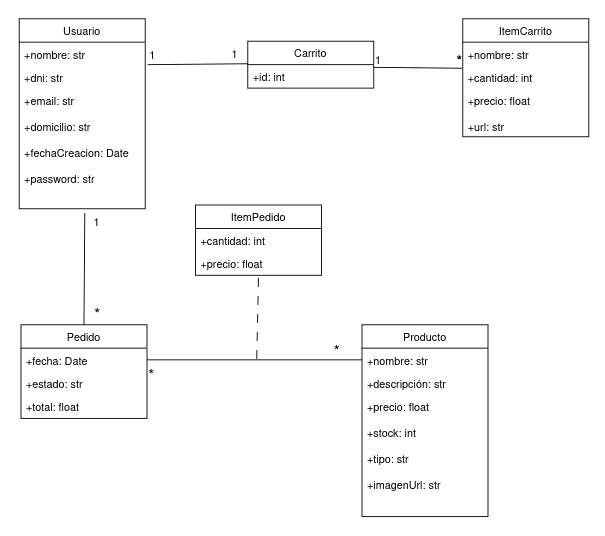
\includegraphics[width=0.75\linewidth]{modeloDom.png}
           \caption{Enter Caption}
           \label{fig:enter-label}
       \end{figure}
        
\subsection{Mapa del sitio web}
    \begin{figure}[H]
        \centering
        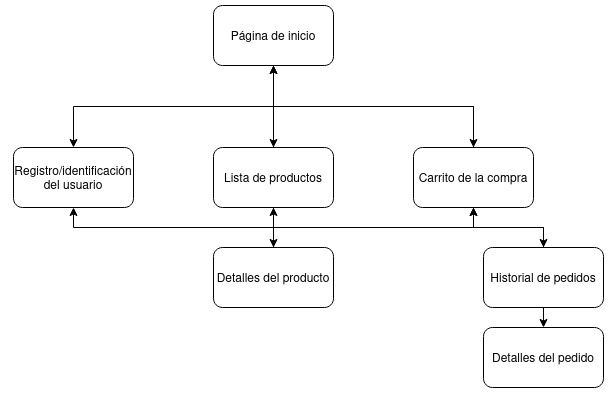
\includegraphics[width=0.70\linewidth]{webM.png}
        \caption{Enter Caption}
        \label{fig:enter-label}
    \end{figure}

\newpage
\section{API}
    \textbf{API (Application Programming Interface)}, Interfaz de Programación de Aplicaciones, es un conjunto de reglas y protocolos que permiten que diferentes programas software se comuniquen e intercambien información entre sí, sin necesidad de que el usuario final sepa los detalles internos de cómo funcionan estas aplicaciones. Es como un puente o traductor que permite que una aplicación le pida cosas a otra de forma controlada y entendible para ambas.\\
    Los \textbf{tipos} de API son:
        \begin{itemize}
            \item Según su acceso:
            \begin{itemize}
                \item APIs abiertas (públicas): cualquier persona puede usarlas sin autenticación.
                \item APIs restringidas (privadas): solo pueden usarlas ciertas aplicaciones o usuarios.
            \end{itemize}
            \item Según su arquitectura:
            \begin{itemize}
                \item RESTful APIs: usan HTTP y recursos estructurados como URLs.
                \item SOAP: usan XML.
            \end{itemize}
        \end{itemize}
    Los \textbf{principales usos} de las APIs son:
        \begin{itemize}
            \item Integración de servicios: permiten que diferentes servicios web y aplicaciones se conecten y compartan funcionalidades.
            \item Desarrollo de aplicaciones modulares: son aplicaciones complejas divididas en módulos.
            \item Acceso a datos y funcionalidades: exponen datos y funcionalidades específicas de una aplicación.
            \item Automatización de tareas: permiten automatizar tareas para que no sea necesario la intervención humana.
            \item Creación de nuevas aplicaciones y servicios: combinando funcionalidades de diferentes sistemas de manera sencilla.
            \item Plataformas como servicio (PaaS): plataformas en la nube.
            \item Microservicios: funcionalidades pequeñas en la arquitectura de microservicios.
        \end{itemize}
    Existen diferentes \textbf{métodos} HTTP, que son utilizados por las APIs:
        \begin{itemize}
            \item GET: usado para obtener datos del servidor.
            \item POST: usado para enviar datos al servidor y crear un nuevo recurso.
            \item PUT: usado para reemplazar completamente un recurso existente.
            \item PATCH: usado para actualizar parcialmente un recurso.
            \item DELETE: usado para eliminar un recurso.
        \end{itemize}

    \subsection{Endpoints de la práctica}
        \begin{itemize}
            \item Autenticación (Login y Registro)
            \begin{itemize}
                \item \textbf{POST /api/login} $\rightarrow$ verificar credenciales y devuelve un token o sesión.
                \item \textbf{POST /api/registro} $\rightarrow$ crea una nueva cuenta de usuario.
                \item \textbf{DELETE /api/logout} $\rightarrow$ cierra sesión de un usuario y eleimina su token.
            \end{itemize}
            \item Menú principal
            \begin{itemize}
                \item \textbf{GET /api/menu} $\rightarrow$ devuelve información general de la tienda y categorías de productos.
            \end{itemize}
            \item Selector de productos
            \begin{itemize}
                \item \textbf{GET /api/productos} $\rightarrow$ devuelve la lista de productos disponibles.
                \item \textbf{GET /api/productos/{id}} $\rightarrow$ devuelve detalles de un producto específico.
            \end{itemize}
            \item Carrito de compra
            \begin{itemize}
                \item \textbf{POST /api/carrito/agregar} $\rightarrow$ agregar un producto al carrito.
                \item \textbf{GET /api/carrito} $\rightarrow$ obtiene el estado actual del carrito.
                \item \textbf{DELETE /api/carrito/vaciar} $\rightarrow$ vacía el carrito del usuario.
            \end{itemize}
            \item Listado de pedidos
            \begin{itemize}
                \item \textbf{GET /api/pedidos} $\rightarrow$ devuelve la lista de pedidos del usuario autenticado.
                \item \textbf{GET /api/pedidos/{id}} $\rightarrow$ devuelve los detalles de un pedido específico.
            \end{itemize}
            \item Proceso de compra
            \begin{itemize}
                \item \textbf{POST /api/checkout} $\rightarrow$ procesa la compra y registra la venta.
            \end{itemize}
            \item Actualización de productos
            \begin{itemize}
                \item \textbf{PUT /api/productos/{id}} $\rightarrow$ actualiza completamente un producto.
                \item \textbf{PATCH /api/productos/{id}} $\rightarrow$ modifica parcialmente un producto.
            \end{itemize}
        \end{itemize}
        
\section{Scripts de nuestra web}
A continuación se detallan una serie de scripts necesarios para arrancar una aplicación web con Flask, junto con otros scripts que ayudan a entender cómo funciona nuestra web.
\subsection{Archivo \texttt{run.py}}

    El archivo \texttt{run.py} actúa como punto de entrada de la aplicación. Este script debe ejecutarse con el entorno virtual activado, utilizando el comando:
    
    \begin{lstlisting}[style=simplebash]
    python run.py
    \end{lstlisting}
    
    Esto lanza el servidor de desarrollo de Flask, cargando todas las plantillas HTML, controladores y rutas definidas en la aplicación.
    
    A continuación, se muestra el contenido del archivo \texttt{run.py}:
    
    \begin{lstlisting}[style=pythonclean, caption={Script principal \texttt{run.py}}]
    from app import create_app
    from flask import render_template, redirect, url_for
    # Crear la aplicación usando la función de fábrica
    app = create_app()
    @app.route('/')
    def hello_world():
        return redirect(url_for('menu.api_index'))  # Redirección a la página principal del menú

    # Filtro personalizado para sumar días a una fecha
    def sumar_dias(fecha, dias):
        from datetime import timedelta
        return fecha + timedelta(days=dias)
    # Registro del filtro en el entorno Jinja
    app.jinja_env.filters['suma_dias'] = sumar_dias

    if __name__ == '__main__':
        app.run(debug=False)
    \end{lstlisting}
    
    Este script realiza las siguientes funciones clave:
    
    \begin{itemize}
      \item Llama a la función \texttt{create\_app()} para crear la instancia de Flask.
      \item Define la ruta principal \texttt{/}, que redirige a la función \texttt{api\_index} del blueprint del menú.
      \item Registra un filtro personalizado en Jinja llamado \texttt{suma\_dias}, útil para mostrar fechas manipuladas en las plantillas.
      \item Inicia el servidor en modo \texttt{debug}. En producción el modo \texttt{debug = False} 
    \end{itemize}
    
\subsection{Archivo \texttt{\_\_init\_\_.py}}
    
    El archivo \texttt{\_\_init\_\_.py} se encarga de inicializar la aplicación Flask, registrar los distintos \textit{blueprints} correspondientes a las funcionalidades de la aplicación y establecer los manejadores de errores.
    
    \begin{lstlisting}[style=pythonclean, caption={Inicialización de la aplicación Flask}]
    from flask import Flask, render_template
    
    def create_app():
        app = Flask(__name__, template_folder='templates')
        app.secret_key = 'clave-super-secreta-123'
        
        # Importación de los blueprints
        from .routes.autentificar import autentificar_usuarios
        from .routes.carritoController import carrito
        from .routes.menuController import menu
        from .routes.pedidoController import pedido
        from .routes.productosController import producto
    
        # Registro de blueprints
        app.register_blueprint(autentificar_usuarios)
        app.register_blueprint(carrito)
        app.register_blueprint(menu)
        app.register_blueprint(pedido)
        app.register_blueprint(producto)
    
        # Registro de manejadores de errores
        register_error_handlers(app)
    
        return app
    
    # Manejadores de errores personalizados
    def register_error_handlers(app):
        @app.errorhandler(400)
        def error400(error):
            return render_template('error.html', error=400, mensaje="No se pudo procesar la petición."), 400
    
        .... Más errores
    \end{lstlisting}
    
    Este archivo realiza las siguientes tareas:
    
    \begin{itemize}
      \item Crea una instancia de Flask con una carpeta de plantillas personalizada.
      \item Establece una clave secreta para el manejo de sesiones.
      \item Registra los \textit{blueprints} correspondientes a las rutas del sistema (autenticación, carrito, menú, pedidos, productos).
      \item Define y registra funciones para manejar errores HTTP comunes, como \texttt{400}, \texttt{401}, \texttt{404} y \texttt{500}, mostrando una plantilla HTML con mensajes personalizados.
    \end{itemize}
\subsection{Blueprints y Organización de Controladores}

Para mantener una estructura modular y organizada, se ha utilizado el sistema de \texttt{Blueprints} de Flask. Cada controlador se define como un módulo independiente que se registra en la aplicación principal a través del archivo \texttt{\_\_init\_\_.py}.

A continuación, se describen los distintos \texttt{Blueprints} definidos:

\begin{itemize}
    \item \texttt{autentificar\_usuarios = Blueprint('autentificar', \_\_name\_\_, url\_prefix="/api")}
    \begin{itemize}
        \item $\rightarrow$ Este blueprint gestiona el controlador de autenticación (\textbf{autentificar}).
        \item $\rightarrow$ Maneja rutas como \texttt{/api/login} y \texttt{/api/registro}.
        \item $\rightarrow$ Se encuentra definido en \texttt{routes/autentificar.py}.
    \end{itemize}

    \item \texttt{carrito = Blueprint('carritoController', \_\_name\_\_, url\_prefix="/api/carrito")}
    \begin{itemize}
        \item $\rightarrow$ Corresponde al controlador de carrito de compras.
        \item $\rightarrow$ Define rutas como \texttt{/api/carrito/agregar}, etc.
        \item $\rightarrow$ Archivo: \texttt{routes/carritoController.py}.
    \end{itemize}

    \item \texttt{menu = Blueprint('menu', \_\_name\_\_, url\_prefix="/api/menu")}
    \begin{itemize}
        \item $\rightarrow$ Controlador encargado de servir los platos del menú.
        \item $\rightarrow$ Ruta base: \texttt{/api/menu}.
        \item $\rightarrow$ Ubicación: \texttt{routes/menuController.py}.
    \end{itemize}

    \item \texttt{pedido = Blueprint('pedidoController', \_\_name\_\_, url\_prefix="/api")}
    \begin{itemize}
        \item $\rightarrow$ Controlador para realizar y gestionar pedidos.
        \item $\rightarrow$ Rutas como \texttt{/api/checkout}, etc.
        \item $\rightarrow$ Se encuentra en \texttt{routes/pedidoController.py}.
    \end{itemize}

    \item \texttt{producto = Blueprint('producto', \_\_name\_\_, url\_prefix="/api")}
    \begin{itemize}
        \item $\rightarrow$ Gestiona los productos de la base de datos.
        \item $\rightarrow$ Rutas típicas: \texttt{/api/productos}, \texttt{/api/productos/<idProducto>}, etc.
        \item $\rightarrow$ Archivo correspondiente: \texttt{routes/productosController.py}.
    \end{itemize}
\end{itemize}

Todos estos \texttt{Blueprints} se registran en la función \texttt{create\_app()} del archivo \texttt{\_\_init\_\_.py} para que formen parte del sistema general de rutas de la aplicación.

\subsection{Decorador \texttt{verificar\_token}} \label{sec:token}

El sistema de autenticación de usuarios se basa en tokens JWT (JSON Web Token) almacenados en cookies. Para proteger rutas que requieren autenticación, se implementa un decorador llamado \texttt{verificar\_token}. Este decorador se aplica a las funciones que sólo deben ser accesibles por usuarios autenticados.

El decorador realiza las siguientes funciones:

\begin{itemize}
    \item Verifica si existe una cookie llamada \texttt{authToken}.
    \item Si el token existe, intenta decodificarlo utilizando una clave secreta y el algoritmo definido.
    \item Si el token es válido, extrae el \texttt{usuario\_id} y lo pasa como argumento a la función decorada.
    \item Si el token ha expirado, borra la cookie y redirige al usuario al formulario de inicio de sesión.
    \item Si el token es inválido o no está presente, se devuelve un error o se redirige al login. El token tiene un tiempo de expiración de 40 minutos; una vez transcurrido este tiempo, si se intenta realizar alguna acción, se devolverá un código 401. Si el token no existiera desde el principio, se devolvería un código de error entre el 300 y el 308. 
    
    Esta lógica podría haber sido distinta, por ejemplo, manejando más la parte del frontend y devolviendo también un error 401. Sin embargo, dado que se quería investigar más a fondo Flask, se implementó de esta manera, redirigiendo desde el backend en lugar de hacerlo desde el frontend. 
    
    Debido a esto, más adelante, en las pruebas de carga (\autoref{sec: locust_err}), se encontrarán errores HTTP entre 300 y 308, y esta es la razón por la que ocurren.
    
\end{itemize}

A continuación, se muestra el código completo del decorador:

\begin{lstlisting}[style=pythonclean, caption={Decorador verificar\_token}]
    def verificar_token(f):
        """
        Decorador que protege rutas requeridas para usuarios autenticados.
        Verifica la validez de un token JWT almacenado en una cookie llamada 'authToken'.
    
        Si el token es válido, extrae el `usuario_id` y lo pasa como primer argumento
        a la función decorada.
    
        - Si el token ha expirado, borra la cookie y redirige al login.
        - Si el token es inválido, devuelve un error JSON 401.
        - Si no hay token, redirige al login.
        """
        @wraps(f)
        def wrapper(*args, **kwargs):
            token = request.cookies.get('authToken')  # Obtener el token de la cookie
            
            if token:
                try:
                    # Intentar decodificar el token
                    token_decode = jwt.decode(token, SECRET, algorithms=[ALGORITHM])
                    usuario_id = token_decode['id']
                    
                    # Llamar a la función original si el token es válido
                    return f(usuario_id, *args, **kwargs)
                
                except jwt.ExpiredSignatureError:
                    # Si el token ha expirado, borra la cookie y redirige al login
                    resp = make_response(redirect(url_for('autentificar.login')))
                    resp.set_cookie('authToken', '', expires=0)
                    return resp
                
                except jwt.InvalidTokenError:
                    # Si el token es inválido
                    return jsonify({"message": "Token inválido"}), 401
            else:
                # Si no hay token, redirige al login
                return redirect(url_for('autentificar.login'))
        
        return wrapper
\end{lstlisting}

Este decorador es esencial para garantizar que sólo los usuarios autenticados puedan acceder a determinadas rutas, especialmente aquellas relacionadas con el carrito, pedidos y perfil de usuario.

\subsection{Ejemplo de Endpoint Protegido con Token}

Uno de los puntos clave de esta práctica ha sido asegurar los endpoints que requieren autenticación mediante el uso de tokens JWT almacenados en cookies. A continuación, se muestra un ejemplo claro de cómo se ha aplicado esta lógica de seguridad:

\begin{lstlisting}[style=pythonclean, caption={Endpoint protegido para mostrar el carrito}]
@carrito.route('/', methods=['GET'])
@verificar_token
def get_items_carrito(usuario_id):
    """
    Muestra los productos actuales en el carrito del usuario autenticado.

    Args:
        usuario_id (int): ID del usuario autenticado extraído del token.

    Returns:
        Response: Renderiza la plantilla del carrito con los productos y el total si existe,
        o la plantilla de inicio con un mensaje de error si el carrito no fue encontrado.
    """

    carrito = get_carrito_items_usuario(usuario_id)
    if isinstance(carrito, Carrito):
        total_carrito = carrito.getTotalCarrito()
        items_json = [item_carrito_schema(item, True) for item in carrito.items]
        
        return render_template("carrito.html", items=items_json, total=total_carrito)

    return render_template("index.html", error="Carrito no encontrado", items=[], total=0)
\end{lstlisting}

\textbf{Explicación del funcionamiento:}
\begin{itemize}
    \item Este endpoint pertenece al \textbf{controlador \texttt{carritoController}}, encargado de gestionar la lógica del carrito de compras.
    \item Utiliza el decorador \texttt{@verificar\_token} para proteger la ruta, exigiendo que el usuario esté autenticado.
    \item El decorador extrae el \texttt{usuario\_id} directamente del token JWT almacenado en la cookie \texttt{authToken}.
    \item Una vez autenticado, se llama a la función \texttt{get\_carrito\_items\_usuario()} que recupera el carrito asociado a ese usuario.
    \item Si el carrito existe, se calcula el total, se transforma cada ítem a formato JSON (usando \texttt{item\_carrito\_schema}) y se renderiza la plantilla \texttt{carrito.html}.
    \item En caso de que el carrito no exista, se redirige a la plantilla de inicio con un mensaje de error.
\end{itemize}

\section{Concluiones página web y Flask}
Este patrón de verificación del token se ha aplicado de forma consistente en otros puntos de la aplicación donde se requiere autenticación como agreagr un producto al carrito, visualizar los pedidos, etc. \\

De este modo se asegura la integridad de la web y facilita tareas de seguridad. Con el desarrollo de esta parte del proyecto se ha podido comprobar lo sencillo que resulta crear una página web con la ayuda de un framework como Flask. Gracias a su estructura basada en Blueprints y a una serie de funciones incorporadas por defecto, se ha facilitado notablemente la organización del código y se ha podido adoptar una arquitectura basada en el modelo MVC (Modelo-Vista-Controlador).\\

Asimismo, se ha observado lo accesible que resulta generar páginas HTML dinámicas mediante el uso de Jinja2, lo cual permite integrar lógica y datos directamente en las plantillas de forma clara y eficiente.\\

Por otro lado, como último apartado de las especificaciones de la práctica, se requería la gestión de al menos cinco productos sobre los que realizar operaciones como añadir, modificar, etc. En nuestro caso, se han añadido algunos productos más, lo cual ha permitido desarrollar una aplicación web más detallada, visualmente atractiva y funcional.\\

\chapter{Base de datos}
\section{Diagrama de base de datos y especificaciones}
Nuestra aplicación web utiliza una base de datos relacional MySQL. El siguiente diagrama muestra la estructura de la base de datos y las relaciones entre las tablas.
\begin{figure}[!h]
    \centering
    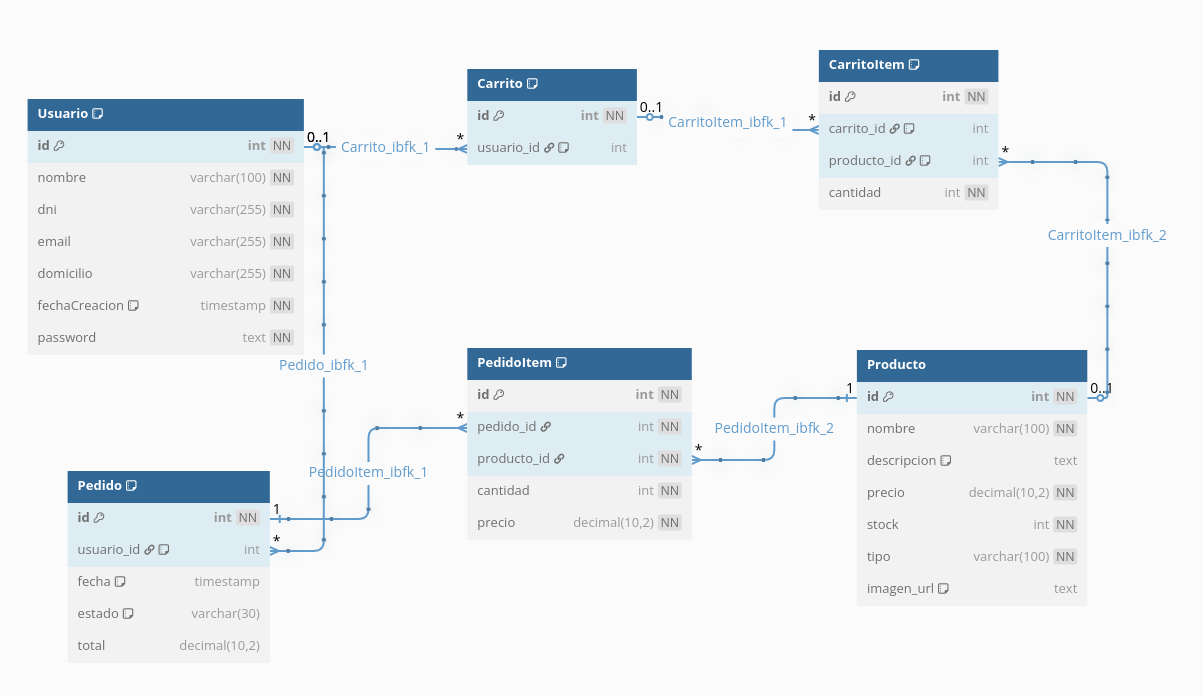
\includegraphics[width=1.05\linewidth]{db.png}
    \caption{Diagrama de base de datos}
    \label{fig:enter-label}
\end{figure}

\subsection{Conexión a la base de datos}

    Para \textbf{iniciar} la base de datos en el servidor, es necesario acceder como root con el comando \lstinline{sudo -i}. A continuación, se deben ejecutar los siguientes pasos:
    
    \begin{enumerate}
        \item \textbf{Acceso a MySQL como root sin usar \texttt{sudo -i}:}
        \begin{itemize}
            \item Ejecutar el comando: \lstinline{sudo mysql -u root -p}
        \end{itemize}
    
        \item \textbf{Creación del usuario \texttt{user\_pr}:}
        \begin{itemize}
            \item Ejecutar el comando: \lstinline{CREATE USER 'user_pr'@'localhost' IDENTIFIED BY 'Grupo6esi';}
            \item Este comando crea un nuevo usuario llamado \texttt{user\_pr} que solo puede conectarse desde el mismo servidor (\texttt{localhost}) y le asigna la contraseña \texttt{Grupo6esi}.
        \end{itemize}
    
        \item \textbf{Creación de la base de datos \texttt{Carga\_web}:}
        \begin{itemize}
            \item Ejecutar el comando: \lstinline{CREATE DATABASE Carga_web;}
            \item Este comando crea una nueva base de datos llamada \texttt{Carga\_web}.
        \end{itemize}
    
        \item \textbf{Selección de la base de datos \texttt{Carga\_web}:}
        \begin{itemize}
            \item Ejecutar el comando: \lstinline{USE Carga_web;}
            \item Este comando selecciona la base de datos \texttt{Carga\_web} para que todas las operaciones posteriores se realicen en ella.
        \end{itemize}
    
        \item \textbf{Ejecución de los scripts SQL para crear las tablas y los procedimientos:}
        \begin{itemize}
            \item Ejecutar: \lstinline{source /home/usuario/esi/PruebasCargawev/srcips_db/creacion_tablas.sql;}
            \item Este archivo contiene las instrucciones para crear las tablas necesarias en la base de datos.
            \item Asegurarse de que el archivo \texttt{creacion\_tablas.sql} existe en la ruta especificada.
            
            \item Ejecutar: \lstinline{source /home/usuario/esi/PruebasCargawev/srcips_db/procedimientos.sql;}
            \item Este archivo contiene las instrucciones para crear los procedimientos almacenados necesarios.
            \item Verificar que el archivo \texttt{procedimientos.sql} esté presente en la ubicación indicada.
        \end{itemize}
        
        \item \textbf{Población de la tabla de productos:}
        \begin{itemize}
            \item Ejecutar: \lstinline{source /home/usuario/esi/PruebasCargawev/srcips_db/insert_productos.sql;}
            \item Este archivo contiene las instrucciones para poblar la tabla de productos con datos de prueba.
            \item Asegurarse de que el archivo \texttt{insert\_productos.sql} existe en la ruta especificada.
        \end{itemize}
        \item \textbf{Cargar toda la base de datos}: Si se quisiera cargar toda la base de datos tblas, procedimientos y población de datos, habría que ejecutar  \lstinline{source /home/usuario/esi/PruebasCargawev/srcips_db/carga_web_dump.sql;}
        
        \item \textbf{Otorgar privilegios al usuario \texttt{user\_pr}:}
        \begin{itemize}
            \item Ejecutar el comando: \lstinline{GRANT ALL PRIVILEGES ON Carga_web.* TO 'user_pr'@'localhost';}
            \item Este comando otorga al usuario \texttt{user\_pr} permisos completos sobre la base de datos \texttt{Carga\_web}, necesarios para leer e insertar datos.
        \end{itemize}
    
        \item \textbf{Actualizar los privilegios:}
        \begin{itemize}
            \item Ejecutar el comando: \lstinline{FLUSH PRIVILEGES;}
            \item Este comando recarga los privilegios de MySQL para aplicar los cambios inmediatamente.
        \end{itemize}
        \item \textbf{Especificaciones:} Este ejemplo para cargar la base de datos se llevaría a cabo descargando la carpeta del proyecto y guardándola en una ruta local. A continuación, sería necesario cambiar la ruta de los comandos dependiendo de dónde se haya guardado dicha carpeta.
        
    \end{enumerate}

        
\subsection{Descripción y relaciones entre tablas}

    La base de datos del sistema está compuesta por seis tablas principales: \texttt{Usuario}, \texttt{Producto}, \texttt{Carrito}, \texttt{CarritoItem}, \texttt{Pedido} y \texttt{PedidoItem}. A continuación, se detalla el propósito de cada tabla y las relaciones que mantienen entre ellas.
    
    \begin{itemize}
        \item \textbf{Usuario}: Almacena la información de los usuarios registrados en el sistema. Cada usuario tiene un \texttt{id} único, y se registran datos como el \texttt{nombre}, \texttt{DNI}, \texttt{email}, \texttt{domicilio}, y \texttt{password}. Además, se guarda la \texttt{fechaCreacion} con una marca de tiempo actualizada automáticamente. Esta tabla está relacionada con las tablas \texttt{Carrito} y \texttt{Pedido}, ya que un usuario puede tener varios carritos o pedidos asociados.
        
        \item \textbf{Producto}: Contiene todos los productos disponibles para ser añadidos al carrito o incluidos en un pedido. Incluye campos como \texttt{nombre}, \texttt{descripcion}, \texttt{precio}, \texttt{stock}, \texttt{tipo} (para clasificar los productos) y \texttt{imagen\_url}. Esta tabla está relacionada con \texttt{CarritoItem} y \texttt{PedidoItem}, permitiendo identificar qué productos se añaden al carrito o se incluyen en un pedido.
        
        \item \textbf{Carrito}: Representa el carrito de compras temporal de un usuario antes de confirmar un pedido. Cada carrito está relacionado con un único usuario mediante \texttt{usuario\_id}. Al eliminar un usuario, sus carritos asociados se eliminan automáticamente (\texttt{ON DELETE CASCADE}).
        
        \item \textbf{CarritoItem}: Registra los productos que un usuario ha añadido a su carrito. Contiene claves foráneas hacia \texttt{Carrito} y \texttt{Producto}, e incluye campos como \texttt{nombre}, \texttt{cantidad} y \texttt{precio}. Cada combinación \texttt{carrito\_id} y \texttt{producto\_id} debe ser única, es decir, no puede haber dos líneas iguales con el mismo producto en el mismo carrito.
        
        \item \textbf{Pedido}: Almacena información sobre los pedidos realizados por los usuarios. Contiene una relación con \texttt{Usuario} a través de \texttt{usuario\_id}. Incluye también la \texttt{fecha} de creación y el \texttt{estado} del pedido (por ejemplo, pendiente, enviado, completado, etc.).
        
        \item \textbf{PedidoItem}: Detalla los productos incluidos en un pedido. Se relaciona con la tabla \texttt{Pedido} mediante \texttt{pedido\_id} y con \texttt{Producto} mediante \texttt{producto\_id}. Almacena la \texttt{cantidad} y el \texttt{precio} con que fue adquirido el producto en ese pedido, permitiendo un historial consistente aunque el precio cambie posteriormente en la tabla \texttt{Producto}.
    \end{itemize}
    
    \subsubsection*{Relaciones entre tablas}
    
    \begin{itemize}
        \item \texttt{Usuario} $\rightarrow$ \texttt{Carrito} (1:N): Un usuario puede tener varios carritos, pero un carrito solo puede pertecer a un usaurio.
        \item \texttt{Usuario} $\rightarrow$ \texttt{Pedido} (1:N): Un usuario puede haber realizado varios pedidos.
        \item \texttt{Carrito} $\rightarrow$ \texttt{CarritoItem} (1:N): Cada carrito puede contener múltiples productos.
        \item \texttt{Pedido} $\rightarrow$ \texttt{PedidoItem} (1:N): Cada pedido puede contener varios productos.
        \item \texttt{Producto} $\rightarrow$ \texttt{CarritoItem} y \texttt{PedidoItem} (1:N): Un producto puede estar presente en múltiples carritos o pedidos.
    \end{itemize}
    
    Estas relaciones permiten modelar un sistema de compras en línea completo, desde la navegación y selección de productos hasta la confirmación del pedido y su almacenamiento.
    
\subsection{Procedimientos almacenados}

\subsubsection{Procedimiento \texttt{AddOrUpdateItemCarrito}}

    Este procedimiento se encarga de \textbf{gestionar los ítems del carrito de compra} de un usuario. Su funcionamiento permite que si un producto ya existe en el carrito, se actualice la cantidad; y si no existe, se inserte como un nuevo ítem.
    
    \begin{itemize}
        \item \textbf{Parámetros de entrada:}
        \begin{itemize}
            \item \texttt{p\_carrito\_id}: ID del carrito.
            \item \texttt{p\_producto\_id}: ID del producto.
            \item \texttt{p\_cantidad}: Cantidad del producto.
        \end{itemize}
        
        \item \textbf{Funcionamiento:}
        \begin{enumerate}
            \item Se consulta si el producto ya está en el carrito.
            \item Si ya existe, se actualiza la cantidad sumando la nueva cantidad.
            \item Si no existe, se inserta como nuevo ítem en la tabla \texttt{CarritoItem}.
        \end{enumerate}

        \item \textbf{Caso de uso:} se utiliza al añadir productos al carrito desde la aplicación, evitando duplicados y facilitando la actualización.
    \end{itemize}
    \begin{lstlisting}[language=SQL, style=SQL]
        BEGIN
            DECLARE cantidad_existente INT;  -- Variable para almacenar la cantidad existente del producto en el carrito
        
            -- Verificamos si el producto ya está en el carrito
            SELECT cantidad INTO cantidad_existente
            FROM CarritoItem
            WHERE carrito_id = p_carrito_id AND producto_id = p_producto_id;
        
            -- Si el producto ya existe en el carrito, actualizamos la cantidad
            IF cantidad_existente IS NOT NULL THEN
                UPDATE CarritoItem
                SET cantidad = cantidad + p_cantidad  -- Sumamos la cantidad existente con la nueva cantidad
                WHERE carrito_id = p_carrito_id AND producto_id = p_producto_id;
            ELSE
                -- Si el producto no está en el carrito, lo insertamos como nuevo ítem
                INSERT INTO CarritoItem (carrito_id, producto_id, cantidad)
                VALUES (p_carrito_id, p_producto_id, p_cantidad);  -- Insertamos los datos proporcionados
            END IF;
        END;
    \end{lstlisting}
\subsubsection{Procedimiento \texttt{CreateUser}}

    Este procedimiento permite \textbf{crear un nuevo usuario en la base de datos}, asegurando que la operación sea atómica gracias a una transacción.
    
    \begin{itemize}
        \item \textbf{Parámetros de entrada:}
        \begin{itemize}
            \item \texttt{p\_nombre}: Nombre del usuario.
            \item \texttt{p\_dni}: DNI del usuario.
            \item \texttt{p\_email}: Correo electrónico del usuario.
            \item \texttt{p\_domicilio}: Domicilio del usuario.
            \item \texttt{p\_password}: Contraseña del usuario.
        \end{itemize}
        
        \item \textbf{Funcionamiento:}
        \begin{enumerate}
            \item Se inicia una transacción.
            \item Se inserta el usuario en la tabla \texttt{Usuario}.
            \item Se recupera el ID del nuevo usuario insertado.
            \item Se hace \texttt{COMMIT} para confirmar los cambios.
            \item Si ocurre un error, se ejecuta un manejador que realiza \texttt{ROLLBACK} y lanza un mensaje de error.
        \end{enumerate}
        
        \item \textbf{Caso de uso:} se ejecuta al registrar un nuevo usuario desde la aplicación. Garantiza que no se guarden datos parciales si algo falla.
    \end{itemize}
    \begin{lstlisting}[language=SQL, style=SQL]
        BEGIN
            DECLARE id_U INT;  -- Variable para almacenar el ID del nuevo usuario
            DECLARE EXIT HANDLER FOR SQLEXCEPTION  -- Manejador de excepciones para capturar errores
            BEGIN
                ROLLBACK;  -- Si ocurre un error, deshacemos la transacción
                SIGNAL SQLSTATE '45000'  -- Lanza una señal con el mensaje de error
                SET MESSAGE_TEXT = 'Ocurrió un error durante la transacción.';  -- Mensaje de error personalizado
            END;
            
            -- Iniciamos la transacción
            START TRANSACTION;
            
            -- Insertamos el nuevo usuario en la tabla Usuario
            INSERT INTO Usuario (nombre, dni, email, domicilio, password)
            VALUES (p_nombre, p_dni, p_email, p_domicilio, p_password);
        
            -- Obtenemos el ID del nuevo usuario insertado
            SET id_U = LAST_INSERT_ID();  -- Recupera el último ID insertado (el del nuevo usuario)
        
            INSERT INTO Carrito (usuario_id) VALUES (id_U);
        
            -- Confirmamos la transacción
            COMMIT;
            
            -- Devolvemos el ID del nuevo usuario
            SELECT id_U AS id;
        END;
    \end{lstlisting}

\chapter{Pruebas de carga con Locust}
\section{Locust} \cite{locust_docs}
    Locust es una herramienta de código abierto escrita en Python para realizar pruebas de carga y rendimiento sobre sitios o aplicaciones web, APIs, o cualquier otro sistema que pueda ser probado mediante peticiones HTTP u otras.\\
    
    Debido a que está desarrollado en Python, lo hace una herramienta flexible, potente y fácil de entender capaz de ser un sistema distribuido y escalable que puede ejecutarse sobre varias máquinas. Además, dispone de una interfaz web en tiempo real que muestra métricas como el número de usuarios activos, número de peticiones por segundo, o tiempos de respuesta y tasas de error.\\
    
    Su principal función es generar tráfico simulado hacia el sistema para medir cómo se comporta bajo diferentes niveles de carga. Otras funcionalidades son:
        \begin{itemize}
            \item Identificar cuellos de botella en el rendimiento.
            \item Evaluar la escalabilidad.
            \item Optimizar el rendimiento.
            \item Planificar la capacidad.
            \item Validar la infraestructura.
            \item Pruebas de estrés.
            \item Pruebas de resistencia.
        \end{itemize}


\subsection{Instalación y Configuración de Locust} 

\cite{locust_video}Para instalar Locust se ha utilizado el siguiente comando:

\begin{lstlisting}[style=simplebash]
    pip install locust
\end{lstlisting}

Para ejecutar las pruebas de carga, se debe lanzar Locust con el siguiente comando:

\begin{lstlisting}[style=simplebash]
    locust -f generar_carga.py --host http://localhost:5000
\end{lstlisting}

En esta práctica se trabaja dentro de un entorno virtual, por lo que es necesario activarlo antes de ejecutar Locust.

Una vez lanzado el comando, se accede a la interfaz web de Locust desde la URL \texttt{http://localhost:8089}, donde se puede configurar el número de usuarios concurrentes y la tasa de aparición.

En nuestro proyecto, el script de Locust se encuentra en la carpeta \texttt{Locust}, ubicada dentro del directorio principal del proyecto. 

Dado que estamos trabajando con el servidor de la universidad, el host utilizado en el comando debe ser:

\begin{center}
\textbf{http://virtual.lab.inf.uva.es:31224}
\end{center}

ya que ahí es donde se encuentra desplegada nuestra aplicación web.

Asimismo, para acceder a la interfaz web de Locust en el entorno remoto, se debe utilizar la siguiente dirección:

\begin{center}
\textbf{http://virtual.lab.inf.uva.es:31223}
\end{center}


\section{Diseño del Script de Carga}  \label{sec:pesos}

El archivo \texttt{generar\_carga.py} define un usuario simulado a través de la clase \texttt{MiUsuario}, que ejecuta varias tareas imitando el comportamiento típico de un usuario real en la tienda online. Estas tareas están agrupadas por funcionalidad, y a cada una se le ha asignado un peso que representa la frecuencia o importancia de su ejecución durante la simulación. A continuación se describe cada grupo de tareas junto con la justificación de su peso:

\begin{itemize}
    \item \textbf{Autenticación}: Incluye el registro y el login de usuarios.  
    El registro se hace solo una vez al crear un nuevo usuario. El login se realiza ocasionalmente, ya que una vez iniciada la sesión, el token permanece activo salvo que expire o se elimine, por lo que su peso es moderado. Las peticiones GET relacionadas también tienen un peso bajo, ya que no son críticas ni frecuentes.

    \item \textbf{Navegación}: Consulta del menú principal y visualización de productos.  
    Ver el menú principal es muy común porque es el punto de entrada a otras secciones, así que tiene peso 2. Ver la lista de productos también es bastante frecuente, ya que la tienda gira en torno a ellos. En cambio, ver los detalles de un producto en específico es menos habitual, así que su peso es 1.

    \item \textbf{Carrito de compras}: Añadir productos, consultar el carrito y vaciarlo.  
    Añadir al carrito es una acción principal dentro de la tienda y genera mucha carga, por eso tiene el peso más alto (3). Consultar o vaciar el carrito se hace menos, así que se les asigna un peso de 1.

    \item \textbf{Checkout}: Proceso de compra y creación de pedidos.  
    Es una tarea crítica porque es donde se concreta la compra. Tiene peso 2, ya que se quiere observar el rendimiento del servidor durante este proceso, pero no se asigna el máximo para evitar una sobre-representación de compras pequeñas, que no serían realistas.

    \item \textbf{Pedidos}: Consulta de pedidos individuales y listados paginados.  
    Son tareas que los usuarios hacen de vez en cuando para verificar sus compras. Por eso, ambas tienen peso 1.

    \item \textbf{Actualización de productos}: Modificaciones completas (PUT) y parciales (PATCH).  
    Aunque no todos los usuarios lo hacen, se quiere ver cómo responde el sistema cuando ocurre. Por eso, ambas tareas tienen peso 2.

    \item \textbf{Gestión de sesión}: Cierre de sesión del usuario.  
    Muchos usuarios no suelen cerrar sesión de forma activa, por lo que esta acción se realiza poco y tiene peso 1. Además era una tarea que no se pedía en el enunciado.
\end{itemize}

\subsection*{Tabla de Pesos Asignados por Tarea}

\begin{center}
\begin{tabular}{|l|c|}
\hline
\textbf{Tarea} & \textbf{Peso} \\
\hline
GET Registro/Login & 1 \\
POST Registro & Se realiza cada vez que se inicia un usuario \\
POST Login & 2 \\
GET Menú Principal & 2 \\
GET Lista de Productos & 2 \\
GET Detalles de Producto & 1 \\
POST Añadir al Carrito & 3 \\
GET Carrito & 1 \\
DELETE Vaciar Carrito & 1 \\
POST Checkout (Compra) & 2 \\
GET Pedido Individual & 1 \\
GET Listado de Pedidos & 1 \\
PUT Producto & 2 \\
PATCH Producto & 2 \\
POST Logout & 1 \\
\hline
\end{tabular}
\end{center}

Esta distribución de pesos busca simular el comportamiento más realista posible de los usuarios dentro de la tienda, dando más peso a las tareas clave como añadir productos o realizar compras, sin descuidar las acciones menos frecuentes pero igualmente importantes para el análisis del rendimiento.

\subsection{Funciones auxiliares}

Para apoyar las tareas de prueba, el script incluye funciones auxiliares importantes:

\begin{itemize}
    \item \texttt{generar\_usuario()}: Crea datos aleatorios para un usuario nuevo, incluyendo nombre, DNI, correo electrónico, domicilio y contraseña.
    \item \texttt{cargar\_json(path)}: Carga un archivo JSON con la lista de productos disponibles para simular acciones sobre productos reales.
\end{itemize}

\subsection{Manejo de autenticación y token}

En el backend de la aplicación, la autenticación está basada en tokens. Para asegurar la validez del token, el backend implementa una función que valida si el token está presente y activo. Si el token falta o ha expirado, el backend responde con redirecciones (códigos HTTP entre 300 y 308) o un código específico 401 (token expirado).

En el script de carga, esta lógica se gestiona en la función \texttt{manejar\_redireccion()}, que interpreta las respuestas del servidor:

\begin{lstlisting}[style=pythonclean, caption={Gestión de redirecciones y expiración de token}]
def manejar_redireccion(self, response, mensaje_ok):
    if response.status_code == 200:
        print(mensaje_ok)
        return True
    elif response.status_code in [301,302,303,307,308]:
        print("❌ Redirigido por problemas con el token")
        return True
    elif response.status_code == 401:
        print("❌ No autorizado: token inválido o expirado (401)")
        return False
    else:
        print(f"❌ Error inesperado ({response.status_code})")
        return False
\end{lstlisting}

Esta función es clave para que las tareas sepan si la petición fue exitosa, si hubo redirección por token inválido o si el token expiró. Así, el script puede reaccionar a cada situación, logrando una simulación realista del flujo de autenticación.


\subsection{Ejemplos de tareas:}

\subsubsection{Agregar producto al carrito (POST /api/carrito/agregar)}

\begin{lstlisting}[style=pythonclean, caption={Tarea para agregar un producto al carrito}]
@task(3)
def agregar_producto_carrito(self):
    if not self.productos_disponibles:
        print("⚠️ No hay productos disponibles.")
        return

    producto = random.choice(self.productos_disponibles)
    data = {"id_producto": producto["id"]}

    with self.client.post("/api/carrito/agregar", json=data, allow_redirects=False, catch_response=True) as response:
        if self.manejar_redireccion(response, "✅ Producto añadido al carrito"):
            response.success()
        else:
            response.failure("❌ Fallo al agregar producto al carrito")
\end{lstlisting}
Esta tarea selecciona un producto aleatorio de la lista cargada desde el archivo \texttt{productos\_cache.json} y lo añade al carrito mediante una petición POST a \texttt{/api/carrito/agregar}


\subsubsection{Registro de usuario (POST /api/registro)}

\begin{lstlisting}[style=pythonclean, caption={Tarea para registrar un nuevo usuario}]
@task(1)
def registro(self):
    data = generar_usuario()
    with self.client.post("/api/registro", json=data, allow_redirects=False, catch_response=True) as response:
        if self.manejar_redireccion(response, "✅ Registro exitoso"):
            self.correo = data["email"]
            self.contrasena = data["password"]
            response.success()
        else:
            response.failure("❌ Error en el registro")
\end{lstlisting}

Esta tarea simula el registro de un nuevo usuario generando datos aleatorios y enviándolos mediante una petición POST. Si el backend responde con una redirección válida o éxito, se almacenan las credenciales para su uso posterior. En el backend existe una función que gestiona tokens; si el token no existe o ha expirado, la aplicación redirige, por eso se comprueban los estados HTTP de redirección (300-308). El código 401 indica que el token ha expirado y se debe iniciar sesión de nuevo.

\subsubsection{Checkout (POST /api/checkout)}

\begin{lstlisting}[style=pythonclean, caption={Tarea para realizar el checkout}]
@task(2)
def checkout(self):
    with self.client.post("/api/checkout", allow_redirects=False, catch_response=True) as response:
        if self.manejar_redireccion(response, "✅ Checkout realizado"):
            if response.status_code == 200:
                pedido = response.json().get("id_pedido")
                if pedido:
                    self.pedido_id = pedido
            response.success()
        else:
            response.failure("❌ Fallo en el checkout")
\end{lstlisting}

Esta tarea simula la finalización de la compra realizando una petición POST al endpoint \texttt{/api/checkout}. Si la respuesta es exitosa y no se requiere redirección, se guarda el identificador del pedido para posibles consultas posteriores. Nuevamente, la verificación del token en el backend asegura que solo usuarios autenticados puedan realizar esta acción.

\subsubsection{Obtener menú (GET /api/menu)}

\begin{lstlisting}[style=pythonclean, caption={Tarea para obtener el menú de productos}]
@task(5)
def obtener_menu(self):
    with self.client.get("/api/menu", allow_redirects=False, catch_response=True) as response:
        if self.manejar_redireccion(response, "✅ Menú obtenido"):
            self.menu = response.json()
            response.success()
        else:
            response.failure("❌ Error al obtener el menú")
\end{lstlisting}

Esta tarea realiza una petición GET para obtener la lista de productos disponibles en el menú. La respuesta se almacena localmente para ser utilizada en otras tareas. Como en los casos anteriores, si el token no está presente o ha expirado, el backend responde con redirección o error para que la simulación controle el flujo de autenticación correctamente.


Este fragmento demuestra cómo se maneja la respuesta para detectar posibles problemas de autenticación o errores del servidor.

\section{Ejecución de la prueba, análisis de resultados}

\subsection{Estrategia de simulación y recogida de métricas}
\cite{xantygc_locust}
Para evaluar el rendimiento del sistema, se llevó a cabo una prueba de carga de 25 minutos utilizando Locust. La ejecución se realizó con el siguiente comando:

\begin{lstlisting}[style=simplebash]
locust -f generar_carga.py -u 180 -r 0.1333 --run-time 25m --host http://virtual.lab.inf.uva.es:31224
\end{lstlisting}

Durante esta prueba se adoptó una metodología estructurada que combinó la simulación progresiva de usuarios, la recolección de métricas técnicas y de negocio, y la visualización periódica de resultados. El enfoque se organizó de la siguiente manera:

\begin{enumerate}
    \item \textbf{Simulación de usuarios:}
    \begin{itemize}
        \item Se simularon hasta 180 usuarios concurrentes realizando acciones comunes: registro, inicio de sesión, consulta del menú, añadido de productos al carrito y checkout.
        \item Cada usuario esperó entre 1 y 3 segundos entre acciones, simulando un comportamiento humano.
        \item La llegada progresiva de usuarios (uno cada 7 segundos) permitió una carga gradual y controlada del sistema.
    \end{itemize}

    \item \textbf{Recogida de métricas técnicas con Grafana:}
    \begin{itemize}
        \item Se monitorizaron continuamente indicadores como uso de CPU, carga del sistema, actividad de E/S, consumo de RAM y frecuencia del procesador.
        \item Esto proporcionó una visión detallada del impacto de la carga sobre el servidor.
    \end{itemize}

    \item \textbf{Métricas de negocio:}
    \begin{itemize}
        \item Se visualizaron en paralelo métricas funcionales como número de pedidos, productos añadidos al carrito y nuevos registros.
        \item Estas métricas, presentadas en Grafana \autoref{sec:visualizacion}, permitieron ver como se relacionaba una experiencia de usuario con el rendimiento del sistema y la web.
    \end{itemize}
\end{enumerate}

\subsection{Captura periódica y análisis de resultados} \label{sec: locust_err}
Con el fin de obtener una visión evolutiva del sistema bajo carga, se implementó una estrategia de muestreo que capturó métricas cada 5 minutos:

\begin{enumerate}
    \item \textbf{Captura periódica automatizada:}
    \begin{itemize}
        \item Se empleó un \textit{event hook} personalizado que registraba estadísticas en un archivo CSV.
        \item También se realizaron capturas manuales desde la interfaz de Locust para asegurar consistencia.
        \item Ambas fuentes de datos fueron combinadas posteriormente en una tabla resumen para análisis.
    \end{itemize}

    \item \textbf{Representatividad de los datos:}
    \begin{itemize}
        \item El muestreo periódico permitió detectar patrones y tendencias generales del sistema.
        \item Como limitación, eventos muy puntuales entre intervalos podrían no haber sido registrados.
        \item Aún así, los datos recopilados fueron suficientes para realizar un análisis global representativo.
    \end{itemize}

    \item \textbf{Indicadores clave desde Locust:}
    \begin{itemize}
        \item Se observaron métricas como el tiempo de respuesta promedio, la tasa de errores, y la cantidad de usuarios activos.
        \item Estas gráficas permitieron identificar posibles cuellos de botella y degradaciones de rendimiento durante la prueba.
    \end{itemize}

    \item \textbf{Tratamiento de errores:}
    \begin{itemize}
        \item Se marcaron como errores los códigos HTTP 3xx y 401, ya que representan fallos en flujos autenticados (como tokens inválidos o sesiones caducadas).
        \item En otros contextos podrían como en casos donde no se requiera de un usuario autenticado, podría considerarse válidos mediante \texttt{success()}, pero para esta prueba se trató como \texttt{failure()} para reflejar una situación más realista.
        \item Como comprobación se adjunta una captura de los errores obtenidos en el análisis donde se puede observar que son errores controlados y que son todos de respuest http de 300 a 308 lo que nos indica que el backend esta funcionando correctamente y que todo va bien como debería ocurrir en casos reales.
        La explicación de estos errores y porque surgen se explican en pasos anteriores (\autoref{sec:token}).
        \newpage

        \begin{figure}[h!]
            \centering
            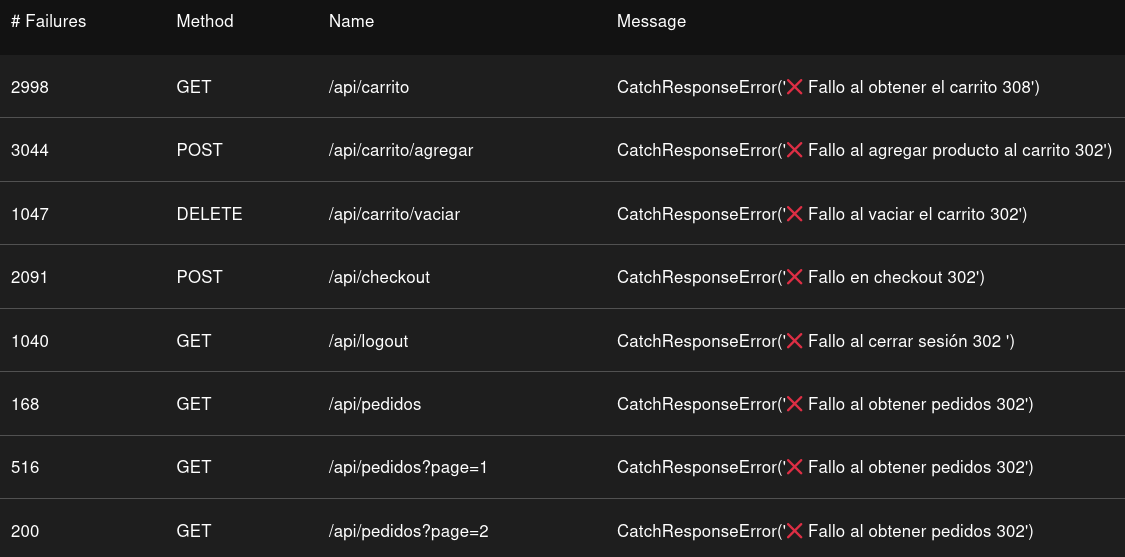
\includegraphics[width=0.95\linewidth]{Fallos.png}
            \caption{Mensajes de fallos previstos en locust}
            \label{fig:enter-label}
        \end{figure}
    \end{itemize}

    \item \textbf{Visualización combinada:}
    \begin{itemize}
        \item Las gráficas de Locust y Grafana mostraron claramente la evolución del sistema frente al aumento progresivo de carga.
        \item Se observó un rendimiento estable con incrementos moderados en los tiempos de respuesta a medida que aumentaban los usuarios.
    \end{itemize}
\end{enumerate}

\subsection*{Análisis resultados}
\noindent A continuación, se incluyen los datos obtenidas cada 5 minutos y algunos ejemplos de como se han obtenido a traves de grafana y la interfaz de locust. En estos resultados se puede apreciar visualmente la evolución del sistema tanto desde la perspectiva técnica (Grafana) como funcional (Locust).



%ejemplo
\begin{itemize}
    \item \textbf{Captura datos minuto 0--5:} \\
    En los primeros 5 minutos, se simularon 41 usuarios concurrentes. 
    
    En Grafana se observa un aumento progresivo del uso de CPU hasta el 20{,}40\%, mientras que la RAM se mantiene estable en torno al 35{,}3\%. La carga del sistema a 1 minuto es de 0{,}30 y la de 5 minutos es de 0{,}12. Ambas se sitúan muy por debajo del umbral crítico de 2, lo que indica que el servidor tiene capacidad de procesamiento disponible.

    \begin{figure}[h!]
        \centering
        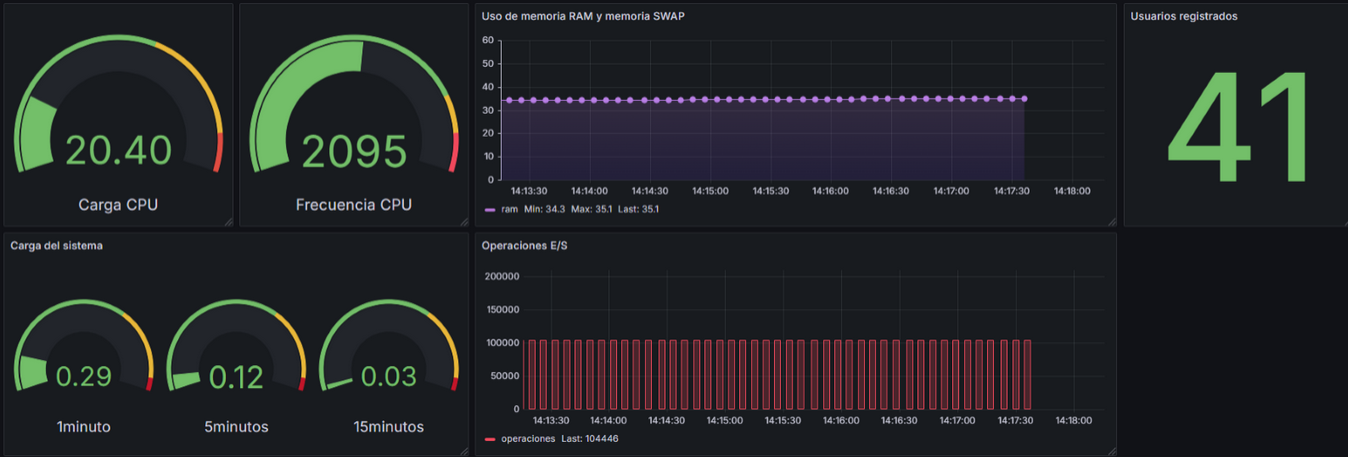
\includegraphics[width=0.7\linewidth]{datos5.png}
        \caption{Datos registrados en el minuto 5}
        \label{fig:enter-label}
    \end{figure}
    El sistema respondió con una media de 16,8 peticiones por segundo y un tiempo de respuesta medio de 134,18\,ms, con un percentil 95 del tiempo de respuesta de 2000\,ms. El número total de peticiones fue de 2753.  No se registraron errores, más que aquellos descritos con anterioridad.
    \begin{figure}[h!]
        \centering
        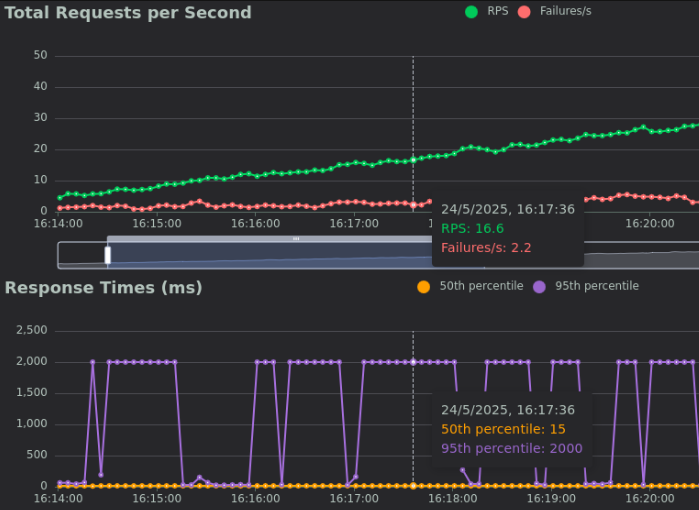
\includegraphics[width=0.65\linewidth]{imagen5.png}
        \caption{Datos de locust registrados en el minuto 5}
        \label{fig:enter-label}
    \end{figure}
    
    \item \textbf{Captura datos minuto 5--10:} \\
    En los siguientes 5 minutos, se simularon 81 usuarios concurrentes. 
    
    En Grafana se observa un aumento del uso de CPU hasta el 30{,}30\%, mientras que la RAM se mantiene estable en torno al 35{,}1\%. La carga del sistema a 1 minuto es de 0{,}36 y la de 5 minutos es de 0{,}33, ambas muy por debajo del umbral de saturación.
    \begin{figure}[h!]
        \centering
        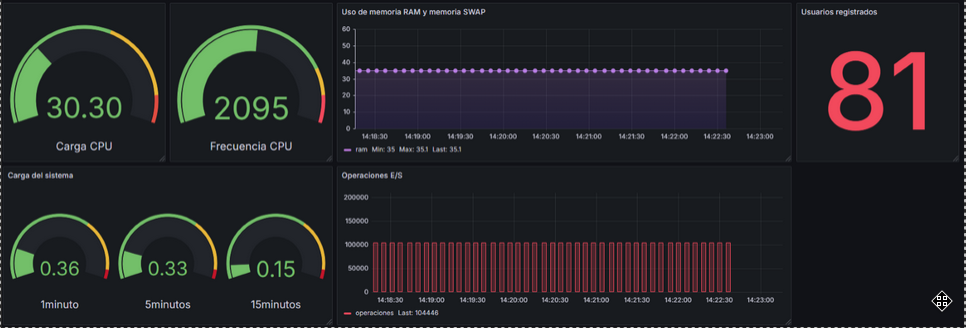
\includegraphics[width=0.7\linewidth]{grafan5.png}
        \caption{Datos registrados en el minuto 10}
        \label{fig:enter-label}
    \end{figure}
    
    El sistema respondió con una media de 35,6 peticiones por segundo y un tiempo de respuesta medio de 132,18\,ms, con un percentil 95 de 2000\,ms. El número total de peticiones fue de 10\,934.  No se registraron errores, más que aquellos descritos con anterioridad.
    \newpage
    \begin{figure}[h!]
        \centering
        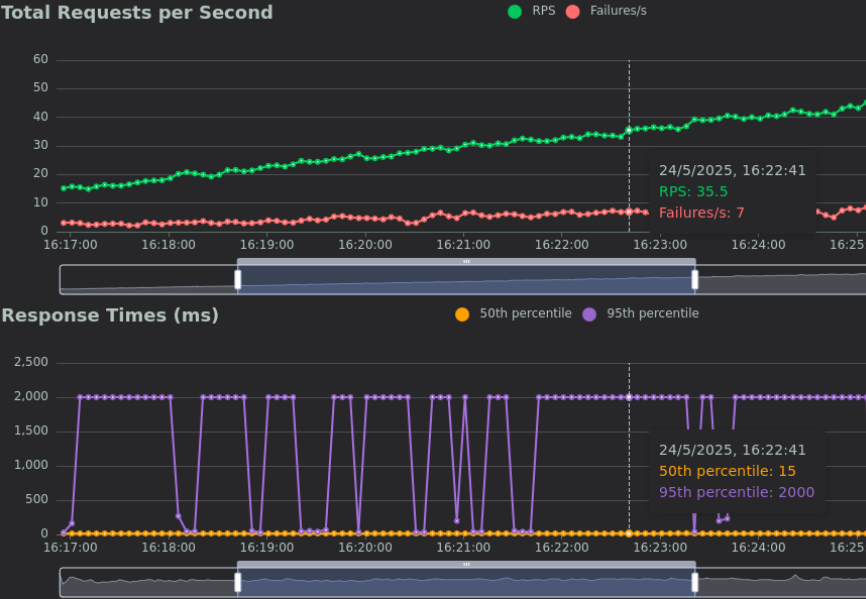
\includegraphics[width=0.65\linewidth]{locust10.png}
        \caption{Datos de locust registrados en el minuto 10}
        \label{fig:enter-label}
    \end{figure}

    \item \textbf{Captura datos minuto 10--15:} \\
    Entre los minutos 10 y 15, se simularon 121 usuarios concurrentes. 
    
    En Grafana se observa un uso de CPU que alcanza el 36{,}40\%, y la RAM se mantiene estable en torno al 34{,}7\%. La carga del sistema a 1 minuto es de 1{,}14 y la de 5 minutos es de 0{,}80. Aunque los valores aumentan, se mantienen por debajo del umbral crítico de 2.
    \begin{figure}[h!]
        \centering
        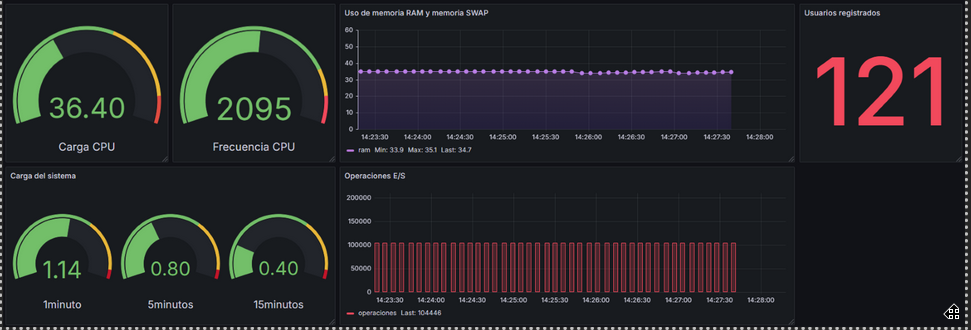
\includegraphics[width=0.75\linewidth]{graf15.png}
        \caption{Datos registrados en el minuto 15}
        \label{fig:enter-label}
    \end{figure}
   
    El sistema respondió con una media de 52,8 peticiones por segundo y un tiempo de respuesta medio de 139,58\,ms, con un percentil 95 de 2000\,ms. El número total de peticiones fue de 24\,217.  No se registraron errores, más que aquellos descritos con anterioridad.
    \begin{figure}[h!]
        \centering
        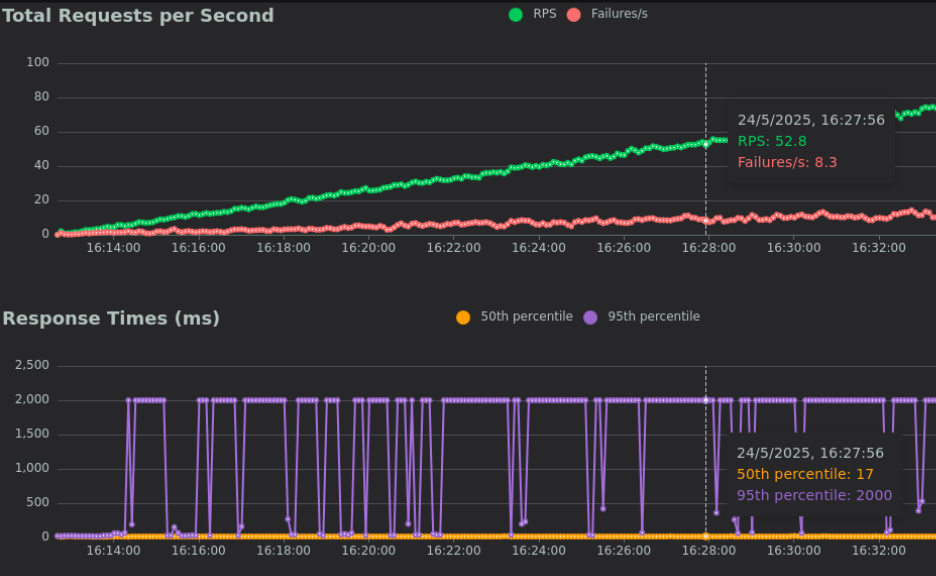
\includegraphics[width=0.65\linewidth]{locust15.png}
        \caption{Datos de locust registrados en el minuto 15}
        \label{fig:enter-label}
    \end{figure}
    \newpage
    \item \textbf{Captura datos minuto 15--20:} \\
    En los siguientes 5 minutos, se simularon 161 usuarios concurrentes. 
    
    En Grafana se observa un incremento del uso de CPU hasta el 37{,}60\%, mientras que la RAM permanece estable en torno al 34{,}8\%. La carga del sistema a 1 minuto es de 1{,}44 y la de 5 minutos es de 1{,}31. Aunque aún por debajo de 2, los valores se acercan al límite, indicando una mayor exigencia sobre el servidor.
    
    El sistema respondió con una media de 71,5 peticiones por segundo y un tiempo de respuesta medio de 145,44\,ms, con un percentil 95 de 2000\,ms. El número total de peticiones fue de 43\,246.  No se registraron errores, más que aquellos descritos con anterioridad.
    \begin{figure}[h!]
        \centering
        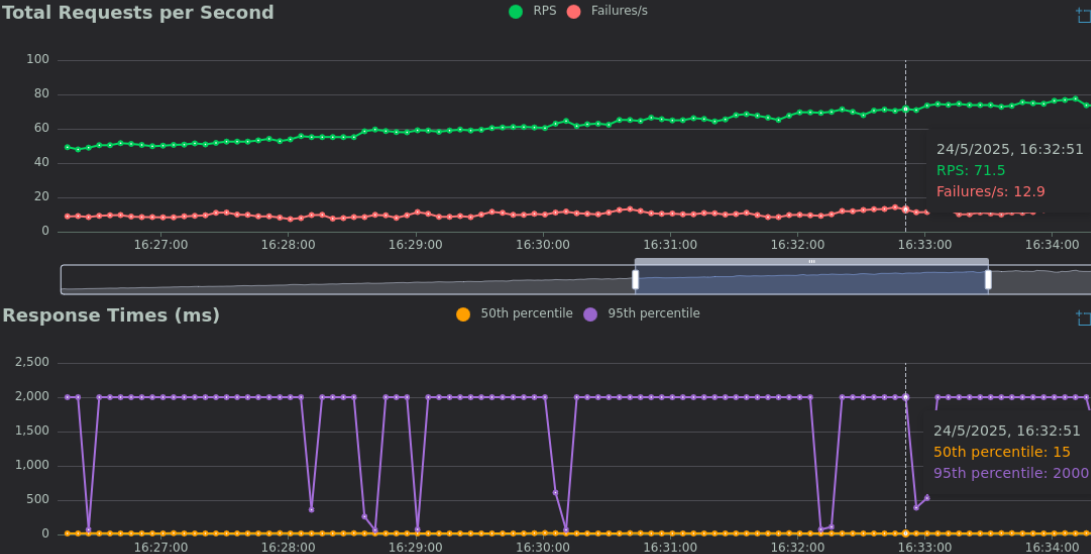
\includegraphics[width=0.75\linewidth]{imagen10_3.png}
        \caption{Datos de locust registrados en el minuto 20}
        \label{fig:enter-label}
    \end{figure}
    \newpage
    \item \textbf{Captura datos minuto 20--25:} \\
    En los últimos 5 minutos, se simularon 180 usuarios concurrentes. 
    
    En Grafana se observa un uso de CPU de hasta el 36{,}40\% y una RAM estable en torno al 34{,}7\%. La carga del sistema a 1 minuto es de 1{,}87 y la de 5 minutos es de 1{,}72, valores que se aproximan al límite crítico, aunque el servidor aún mantiene capacidad disponible.

    El sistema respondió con una media de 79,3 peticiones por segundo y un tiempo de respuesta medio de 149,12\,ms, con un percentil 95 de 2000\,ms. El número total de peticiones fue de 66\,318. No se registraron errores, más que aquellos descritos con anterioridad.
   \item En total se han capturado 66\,318 peticiones, de las cuales 11\,225 han fallado, lo que representa una tasa de error del 16,9\%. El tiempo de respuesta medio ha sido de 149{,}12 ms, con un mínimo de 4 ms y un máximo de 5\,166 ms. El tamaño medio de las respuestas ha sido de 4\,092 bytes. La tasa de peticiones por segundo (RPS) se ha mantenido en torno a 44,2, mientras que la tasa de errores por segundo ha sido de 7,48. 

    A pesar de una media de respuesta aceptable, el número significativo de fallos y la elevada dispersión en los tiempos (especialmente el valor máximo y el percentil 95 cercano a 2\,000 ms) sugieren que existen cuellos de botella, especialmente en endpoints críticos como \texttt{checkout}.El percentil 95 se ha usado con el fín de obtener una referencia del rendimiento general del sistema.

    \begin{figure}[h!]
        \centering
        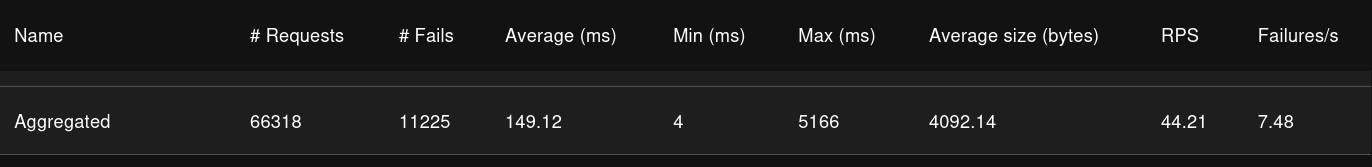
\includegraphics[width=1.0\linewidth]{finalV.png}
        \caption{Resumen final valores Locust}
        \label{fig:enter-label}
    \end{figure}
    
\end{itemize}
\newpage
\subsubsection{Endpoints críticos}

Durante la prueba de carga, se ha podido identificar qué endpoints del sistema son más utilizados y, por tanto, más críticos desde el punto de vista del rendimiento y la estabilidad. El análisis del ratio final y total de peticiones por clase revela una distribución equilibrada entre las diferentes rutas del usuario \texttt{MiUsuario}, pero con algunos puntos especialmente relevantes. Los resultados de este análisis podrían haber sido distintos si se hubiera cambiado el peso de las tareas, pero como se mencionó en el punto (\autoref{sec:pesos}), estos pesos se asignaron de manera que nos parecía coherente y que reflejaba cómo de verdad tenía que actuar nuestra web y sistema en condiciones reales.

\begin{figure}[!h]
    \centering
    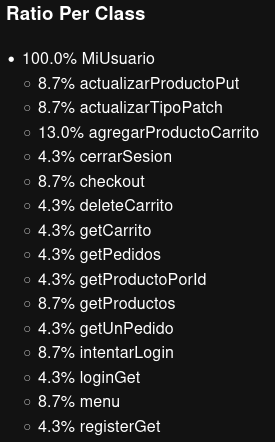
\includegraphics[width=0.30\linewidth]{ratios.png}
    \caption{Ratios por clase}
    \label{fig:enter-label}
\end{figure}

\begin{itemize}
    \item El endpoint \texttt{agregarProductoCarrito} (\texttt{/api/carrito/agregar}) destaca como el más utilizado, con un 13,0\% del total, lo que lo convierte en un candidato prioritario para optimización y pruebas de robustez. Dado que en este endpoint se realizan varias operaciones de base de datos, y con los resultados obtenidos, podría convertirse en un cuello de botella bajo condiciones de estrés como las generadas durante la prueba.

    \item Le siguen varios endpoints con una participación del 8,7\% cada uno: \newline
    \texttt{actualizarProductoPut} ('/api/productos/id'), \texttt{actualizarTipoPatch} ('/api/productos/id'), \texttt{checkout} ('/api/checkout'), \texttt{getProductos} ('/api/productos'), \texttt{intentarLogin} ('/api/login'), \texttt{menu} ('/api/menu'). Esta frecuencia significativa sugiere que deben ser monitorizados en escenarios de carga elevada. En particular, \texttt{checkout} e \texttt{intentarLogin}, que implican varias operaciones internas como validaciones y consultas más extensas a la base de datos, aumentan el riesgo de convertirse en otro cuello de botella. Como se puede observar en los datos recogidos anteriormente, el percentil 95 presenta casi siempre un valor cercano a los 2000 ms. Esto se debe al endpoint de \texttt{checkout},la cual es una función de mucho peso ya que hace varios inserts a base datos y tiene un lógica más pesada, pero además incluye un retraso de 2 segundos, según las especificaciones de la práctica, con el objetivo de simular una transacción real. Entre las peticiones que superan los 2000 ms se encuentran principalmente las del endpoint \texttt{checkout}, como se puede observar en la imagen de abajo, donde se evidencia que este endpoint genera un retraso significativo debido a la simulación de una transacción real con un retardo de 2 segundos. Este comportamiento explica por qué dicho endpoint es tan crítico y cómo su tiempo de respuesta afecta directamente al valor del percentil 95. Dado que se realizaron 66\,318 peticiones en total, esto significa que unas 62\,002 fueron más rápidas o iguales a 2000 ms, mientras que las restantes 4\,316 superaron ese umbral. Por tanto, el endpoint \texttt{checkout} influye de forma directa en la percepción de rendimiento para una parte relevante de los usuarios, lo que puede impactar negativamente en la eficiencia general de la web.
    \begin{figure}[h!]
        \centering
        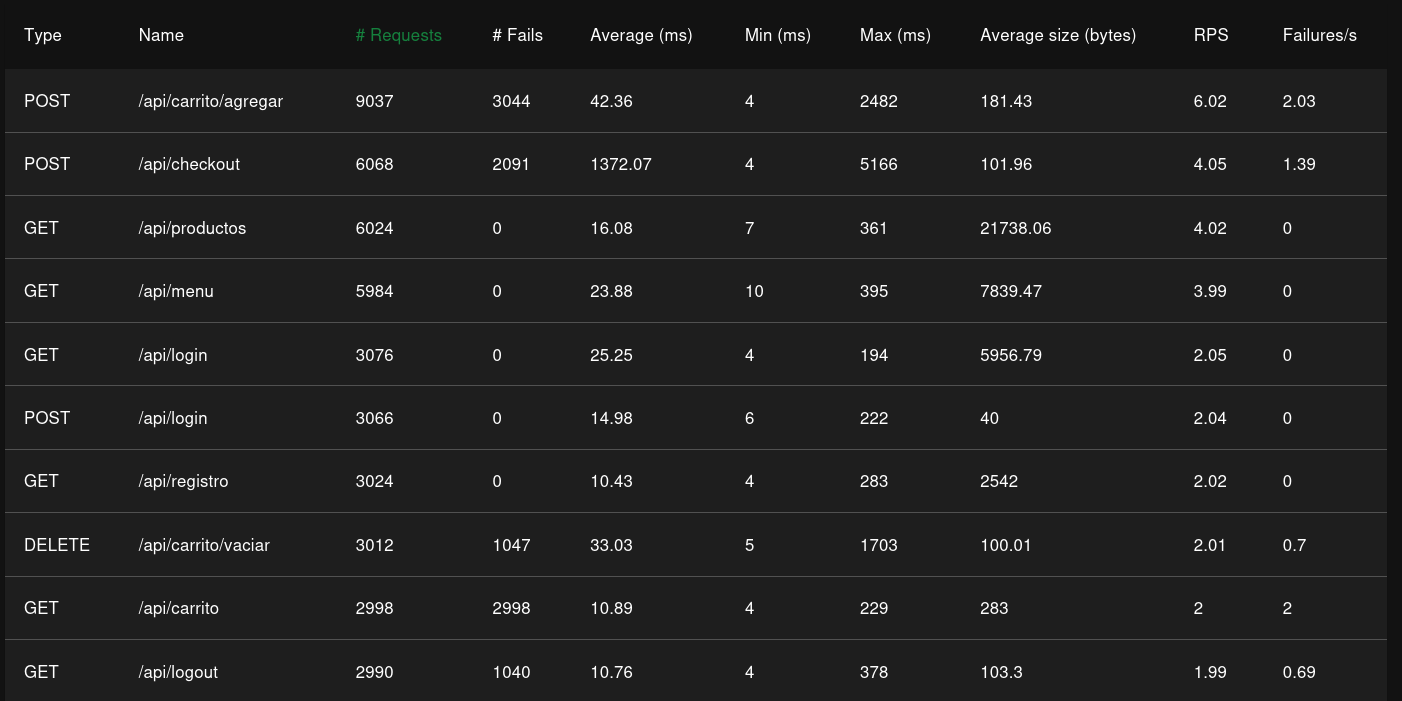
\includegraphics[width=1.0\linewidth]{salidaLF.png}
        \caption{Salida de medición de locust}
        \label{fig:enter-label}
    \end{figure}

    \item Otros endpoints como \texttt{cerrarSesion} ('/api/logout'), \texttt{deleteCarrito} ('/api/carrito/vaciar'),  \texttt{getCarrito} ('/api/carrito'),  \texttt{getPedidos} ('/api/pedidos'), \texttt{getProductoPorId} ('/api/productos/id'), \newline \texttt{getUnPedido} ('/api/pedidos/id'), \texttt{loginGet} ('/api/login') y \texttt{registerGet} ('/api/registro')se mantienen en un 4,3\%, siendo menos críticos individualmente. No obstante, su uso combinado representa una carga significativa y podrían convertirse en un problema si el número de usuarios o la carga aumentara.
\end{itemize}

Este análisis del ratio por clase proporciona una visión clara de dónde se deben realizar pruebas más exhaustivas sobre ciertos endpoints antes de realizar cambios en el código. En particular, los endpoints con ratios superiores al 8\% pueden considerarse como críticos para la experiencia del usuario bajo condiciones reales de uso. Además, aquellos que impliquen operaciones con la base de datos o múltiples pasos internos (como \texttt{agregarProductoCarrito} o \texttt{checkout}) deberían ser revisados para majorar y ofrecer una experiencia de usuario mejor.

\section{Análisis de rendimiento y posibles cuellos de botella}
En esta sección se detalla cómo se ha medido el rendimiento del sistema y cómo éste se comporta ante situaciones de saturación de carga.

A continuación se muestra una tabla resumen con todos los datos recogidos en cada captura:

\begin{table}[H]
\centering
\sisetup{
  output-decimal-marker={,}, 
  table-format=3.2
}
\begin{tabular}{|c|c|c|S[table-format=3.2]|S[table-format=2.2]|S[table-format=2.1]|}
\hline
\textbf{Tiempo (min)} & \textbf{Usuarios} & \textbf{Resp. media (ms)} & \textbf{Peticiones/s} & \textbf{CPU (\%)} & \textbf{RAM (\%)} \\
\hline
0-5   & 41  & 134,18 & 16,8 & 20,40 & 35,3 \\
5-10  & 81  & 132,18 & 35,6 & 30,30 & 35,1 \\
10-15  & 121 & 139,58 & 52,8 & 36,40 & 34,7 \\
15-20  & 161 & 145,44 & 71,5 & 37,60 & 34,8 \\
20-25  & 180 & 149,12 & 79,3 & 36,40 & 34,7 \\
\hline
\end{tabular}
\caption{Resumen de usuarios, tiempo medio de respuesta, peticiones por segundo y uso de recursos}
\label{tab:resumen-recursos}
\end{table}

\begin{table}[H]
\centering
\sisetup{table-format=1.2}
\begin{tabular}{|c|S[table-format=1.2]|S[table-format=1.2]|c|c|}
\hline
\textbf{Tiempo (min)} & \textbf{Carga min 1} & \textbf{Carga min 5} & \textbf{Freq. CPU (MHz)} & \textbf{Operac. E/S} \\
\hline
0-5   & 0,30 & 0,12 & 2095 & 10446 \\
5-10  & 0,36 & 0,33 & 2095 & 10446 \\
10-15  & 1,14 & 0,80 & 2095 & 10446 \\
15-20  & 1,44 & 1,31 & 2095 & 104450 \\
20-25  & 1,87 & 1,72 & 2095 & 104452 \\
\hline
\end{tabular}
\caption{Carga del sistema, frecuencia de CPU y operaciones de E/S durante la prueba de carga}
\label{tab:carga-frecuencia}
\end{table}

\subsection{Rendimiento básico: Throughput y Latencia}

\begin{itemize}
  \item \textbf{Throughput} (o rendimiento): peticiones por segundo (RPS). El throughput crece casi linealmente conforme aumentan los usuarios, hasta los 180 concurrentes.
  
  \item \textbf{Latencia promedio}: tiempo medio que tarda una petición en responderse. La latencia se mantiene bastante estable, entre 130 y 150 ms, con ligeros picos conforme suben los usuarios, lo cual es normal.
\end{itemize}

Con esto podemos decir que el sistema aguanta bien la carga aplicada.

\subsection{Uso de recursos y carga del sistema}

\begin{itemize}
  \item La \textbf{CPU} sube hasta un 37\%, pero no llega ni cerca del 100\%, así que no está saturada.
  
  \item La \textbf{RAM} se mantiene bastante estable, sin cambios significativos.
  
  \item La \textbf{carga promedio} del sistema (load average) llega hasta 1.87 en 1 minuto, lo que indica que hay procesos esperando para ejecutarse, pero sigue siendo menos que el número de núcleos (nuestro sistema cuenta con dos núcleos).
\end{itemize}

En resumen, la \textbf{CPU} podría ser un posible límite en el futuro, pero todavía hay margen.

\subsection{Eficiencia por usuario}

Para saber si el sistema mantiene su rendimiento por usuario, calculamos el throughput por usuario activo:

\[
\text{Throughput por usuario} = \frac{\text{Peticiones por segundo}}{\text{Usuarios concurrentes}}
\]

\begin{table}[H]
\centering
\begin{tabular}{|c|c|c|c|}
\hline
\textbf{Tiempo (min)} & \textbf{Usuarios} & \textbf{Peticiones/s} & \textbf{RPS por usuario} \\
\hline
0-5  & 41  & 16.8  & 0.410 \\
5-10 & 81  & 35.6  & 0.440 \\
10-15 & 121 & 52.8  & 0.436 \\
15-20 & 161 & 71.5  & 0.444 \\
20-25 & 180 & 79.3  & 0.441 \\
\hline
\end{tabular}
\caption{Throughput por usuario durante la prueba}
\end{table}

El \textbf{throughput} por usuario se mantiene casi constante en 0.44 RPS, lo que indica que el sistema escala correctamente y sigue siendo eficiente por usuario. Los recursos se reparten de manera equilibrada.

\subsection{Posibles cuellos de botella}

\begin{itemize}
  \item La \textbf{carga del sistema} se acerca al número de núcleos (1.87 de load average), por lo que si el servidor tiene 2 núcleos, está casi saturado. Esto podría explicar la ralentización en el crecimiento del throughput.
  
  \item La \textbf{CPU} está al 37\%, no saturada, pero el aumento en latencia indica que algunas peticiones pueden estar esperando recursos. Por ahora no es problema, pero si sube la carga, podría ser un cuello de botella.
  
  \item La \textbf{RAM} se mantiene estable, no parece ser un problema.
\end{itemize}

\subsection{Ley de Little}

La \textbf{Ley de Little} establece que el número medio de trabajos en un sistema en equilibrio es igual al producto de la tasa media de llegadas y el tiempo medio de permanencia en el sistema:

\[
Q = \lambda \cdot R
\]

Donde:

\begin{itemize}
    \item \( Q \): número medio de trabajos en el sistema (también llamado población media del sistema),
    \item \( \lambda \): tasa media de llegada (trabajos o peticiones por segundo),
    \item \( R \): tiempo medio que un trabajo permanece en el sistema (en segundos).
\end{itemize}

Para aplicar esta ley, **se debe asumir que el sistema está en equilibrio**, es decir, que la tasa de llegada de trabajos es igual a la tasa de salida. Esto implica que el número de trabajos en el sistema se mantiene estable en el tiempo: por cada trabajo que entra, otro sale.

En nuestro caso, **esta condición de equilibrio se considera válida** porque los usuarios se van generando de forma progresiva a lo largo del tiempo (no todos a la vez), y una vez dentro del sistema, comienzan a realizar tareas como navegar, añadir productos o finalizar compras. Esto permite que el sistema estabilice su comportamiento y alcance un flujo constante de peticiones, simulando una carga realista.

Bajo este equilibrio, se puede reformular la ley como:

\[
N = \mu \cdot R
\]

donde:

\begin{itemize}
    \item \(N\): número de usuarios concurrentes,
    \item \(\mu\): throughput o tasa de procesamiento (peticiones por segundo),
    \item \(R\): tiempo medio de respuesta por petición (en segundos).
\end{itemize}

A continuación, se compara el producto \(\mu \cdot R\) con los valores observados de \(N\):

\begin{table}[H]
\centering
\begin{tabular}{|c|c|c|c|c|}
\hline
\textbf{Tiempo (min)} & \textbf{Usuarios \(N\)} & \textbf{Resp. media \(R\) (s)} & \textbf{Throughput \(\mu\)} & \(\mu \cdot R\) (estimado) \\
\hline
0-5  & 41  & 0.134 & 16.8  & 2.25 \\
5-10 & 81  & 0.132 & 35.6  & 4.71 \\
10-15 & 121 & 0.140 & 52.8  & 7.37 \\
15-20 & 161 & 0.145 & 71.5  & 10.40 \\
20-25 & 180 & 0.149 & 79.3  & 11.82 \\
\hline
\end{tabular}
\caption{Validación de la Ley de Little (R en segundos)}
\end{table}

Como se observa, \(\mu \cdot R\) es menor que \(N\), lo cual indica que no todos los usuarios están activos al mismo tiempo; muchos están esperando o inactivos entre acciones. Esto es coherente con el comportamiento definido en las pruebas, donde los usuarios introducen tiempos de espera de entre 1 y 3 segundos para simular interacciones reales.

\subsection{Conclusiones de los resultados}

Podemos decir que el sistema es eficiente porque:

\begin{itemize}
    \item El throughput crece bastante mientras la CPU sube poco.
    \item El sistema aguanta bien la carga sin saturarse ni que la latencia aumente demasiado.
    \item El percentil 95 nos dice que unas 62 002 peticiones dueron más raṕida o iguales a 2000 ms, y 4316 han superado ese umbral. Por lo que hay enpoints que están causando cuellos de botella. Entre estos endpoint destacar el de relizar un pedido ('checkout'), el cual de entre todas sus petiones no fallidas, casi todas las que han superado el umbral son de este enpoint, como se vio con anterioridad.
    \item Se concluye que no todos los usuarios están activos en cada momento, algunos están en espera entre acciones/tareas.
\end{itemize}

En resumen, el sistema funciona bien hasta 180 usuarios concurrentes, con buen rendimiento y sin cuellos de botella claros todavía.

No obstante, si se continuase aumentando la cantidad de usuarios más allá de este punto, es probable que la \textbf{CPU comience a saturarse}, y como consecuencia, la latencia podría incrementarse rápidamente. Esto se debe a que el sistema estaría operando muy cerca de su \textbf{límite de capacidad}, por lo que pequeñas variaciones en la carga o en la disponibilidad de recursos podrían provocar un comportamiento no lineal, con una caída del rendimiento y aumento del tiempo de respuesta de forma abrupta.

Por tanto, si se desea escalar el sistema para soportar una carga superior, sería recomendable considerar optimizaciones a nivel de backend o infraestructura, como balanceo de carga, caché de contenido o escalado horizontal mediante la distribución de servicios.




\subsection{Mejoras para el Rendimiento Web}
Durante el desarrollo del backend se aplicaron diversas optimizaciones que, en ese momento, se consideraron útiles para mejorar el rendimiento del sistema. Gracias a estas mejoras, es posible que se haya conseguido un mejor comportamiento bajo carga. Entre las principales acciones implementadas destacan:

\begin{itemize}
    \item \textbf{Paginación en los endpoints de pedidos}: Para evitar la carga excesiva de datos al listar muchos pedidos. Se muestran 5 pedidos por página y cada vez que se cambia de página se carga unos nuevos pedido, de esta forma, si un usuario realiza muchos pedidos, la consulta a este endpoint no genera tanta carga y lo irá cargando poco a poco todo.
    \item \textbf{Procedimientos almacenados}: Se han creado en MariaDB para optimizar operaciones como la creación de usuarios o pedidos, reduciendo el número de consultas que realiza la aplicación. Además, para consultas que se ejecutan de forma consecutiva y que no están encapsuladas en un procedimiento almacenado, se utiliza la misma conexión a la base de datos durante todas ellas, cerrándola únicamente al finalizar.
    \item \textbf{Comprobaciones previas a las consultas}: Antes de realizar tareas como modificaciones en los productos, se verifica primero si los datos introducidos son diferentes a los que ya están registrados. Es decir, al intentar modificar un producto, se realiza primero un SELECT para obtener los datos actuales de dicho producto y se comparan con los datos nuevos introducidos. Si los datos son distintos, se ejecuta un UPDATE en la base de datos para actualizar la información; en caso contrario, no se realiza ninguna acción.
    \item \textbf{Minimización de consultas anidadas}: Se han reestructurado algunas funciones para reducir el coste computacional de las consultas complejas, como en el caso de obtener el carrito de un usuario o los productos de un pedido. De esta manera, se consigue un código más escalable y fácil de mantener.
\end{itemize}


\section{Conclusiones pruebas de carga con Locust}
Gracias a Locust, ha sido posible obtener una visión detallada del comportamiento del sistema bajo distintas cargas de trabajo. Esta información, una vez recogida y analizada, resulta muy útil para tomar decisiones informadas de cara a futuras optimizaciones o modificaciones del sistema.\\

La sintaxis basada en Python ha facilitado la creación de escenarios de prueba de forma sencilla y flexible. Una vez comprendido el funcionamiento básico de la herramienta, su uso se vuelve intuitivo y permite analizar múltiples aspectos del rendimiento de la aplicación, como tiempos de respuesta, peticiones por segundo o errores, entre otros.\\

Locust se presenta como una herramienta muy útil para llevar a cabo pruebas de carga.\\


\chapter{Monitorización del servidor con Grafana}
En la práctica anterior se recogieron métricas de rendimiento del servidor como el uso de CPU, memoria RAM, frecuencia de la CPU, operaciones de entrada/salida (E/S), entre otras, las cuales se visualizaron mediante paneles en Grafana. Estas métricas permitieron monitorizar el estado general del sistema durante las pruebas de carga.\\

En esta parte, se han añadido nuevas métricas relacionadas con las reglas de negocio definidas, tales como el número de usuarios registrados, pedidos creados, ingresos totales, número de carritos con ítems dentro y el top 10 de productos más vendidos. Estas métricas permiten evaluar el comportamiento y la carga real de la página web desde un punto de vista más comercial.

\section{Conexión a base de datos desde grafana}
En este punto se detalla cómo conectar Grafana a la base de datos utilizada por la aplicación web y cómo añadir al dashboard creado en la práctica anterior la visualización de las nuevas métricas.

Para ello, accedemos a la sección de Connections y seleccionamos MySQL. A continuación, es necesario introducir los datos de conexión correspondientes y ajustarlos según la configuración de la base de datos.

Una vez creada la conexión y confirmada su correcta configuración, nos dirigimos a la sección de Dashboards, donde seleccionaremos el dashboard creado en la práctica anterior. Dentro de este, accedemos a la opción Edit y pulsamos en Add Visualization para añadir una nueva visualización.

En el apartado de Data source podremos seleccionar la base de datos que deseamos utilizar: puede ser la propia de Grafana, la base de datos de esta práctica, cualquier otra disponible o incluso una combinación (mixed) de dos o más fuentes de datos.

Una vez seleccionada la fuente de datos, ya es posible realizar las consultas necesarias y visualizar los datos en el dashboard.

\section{Reglas de negocio} \cite{metricas_boske}
En este apartado se detallan las métricas de negocio seleccionadas para su visualización.

La elección de estas métricas se ha realizado en base a su relevancia e interés para el análisis de la actividad de la aplicación web, así como por su posible utilidad en un entorno comercial real.

A continuación, se enumeran cinco de las métricas consideradas más representativas:
\begin{itemize}
    \item \textbf{Número de usuarios registrados}: Permite conocer el número de usuarios en tiempo registrados.
    \item \textbf{Pedidos creados}: Refleja el número de transacciones. 
    \item \textbf{Ingresos totales}: Refleja el rendimiento económico.
    \item \textbf{Numero de carritos que tienen items/productos dentro}: Permite conocer los usuarios que podrían estar listo para realizar un pedido.
    \item \textbf{Top 10 productos más vendidos}: Permite evaluar como de eficaz y atractiva es la web y los productos que se venden.
\end{itemize}

\section{Visualización de Grafana}\label{sec:visualizacion}
\subsection*{Número de usuarios registrados en la página web}

Esta métrica se encarga de recolectar el número de usuarios que se han ido generando y registrando en nuestra página web. De esta manera, se puede conocer cuántos usuarios están ejecutando tareas o no, y medir de forma coherente el rendimiento del sistema.

Para ello, dentro de Grafana se ha escrito la siguiente sentencia SQL:

\begin{lstlisting}[language=SQL, style=SQL]
SELECT COUNT(id) FROM Carga_web.Usuario
\end{lstlisting}

Esta consulta se encarga de obtener cuántos usuarios hay registrados en cada momento.

Para mostrarlo en Grafana, se ha optado por una visualización de tipo *Stat*, donde simplemente se pueden ver los usuarios totales registrados en tiempo real.

\begin{figure}[!h]
    \centering
    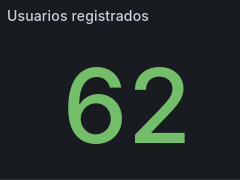
\includegraphics[width=0.3\linewidth]{usuariosreg.png}
    \caption{Usuarios Registrados}
    \label{fig:enter-label}
\end{figure}

\subsection*{Ingresos totales}

Esta métrica está más orientada a la parte comercial, ya que permite visualizar los ingresos totales que la empresa ha generado en un momento dado, así como su evolución a lo largo del tiempo.

Para ello, dentro de Grafana se ha utilizado la siguiente sentencia SQL:

\begin{lstlisting}[language=SQL, style=SQL]
SELECT 
    FROM_UNIXTIME(UNIX_TIMESTAMP(fecha) - MOD(UNIX_TIMESTAMP(fecha), 5)) AS tiempo_agrupado,
    SUM(total) AS ingreso_total
FROM 
    Carga_web.Pedido
WHERE 
    fecha BETWEEN NOW() - INTERVAL 5 MINUTE AND NOW()
GROUP BY 
    tiempo_agrupado
ORDER BY 
    tiempo_agrupado;
\end{lstlisting}

Esta consulta agrupa los ingresos cada 5 segundos, permitiendo visualizar cómo varían con el tiempo. 

Para mostrar los resultados en Grafana, se ha optado por una visualización de tipo *Time series*, que permite observar la evolución de los ingresos en intervalos regulares. Además, se puede obtener el total acumulado de ingresos para el rango de tiempo seleccionado.

\begin{figure}[!h]
    \centering
    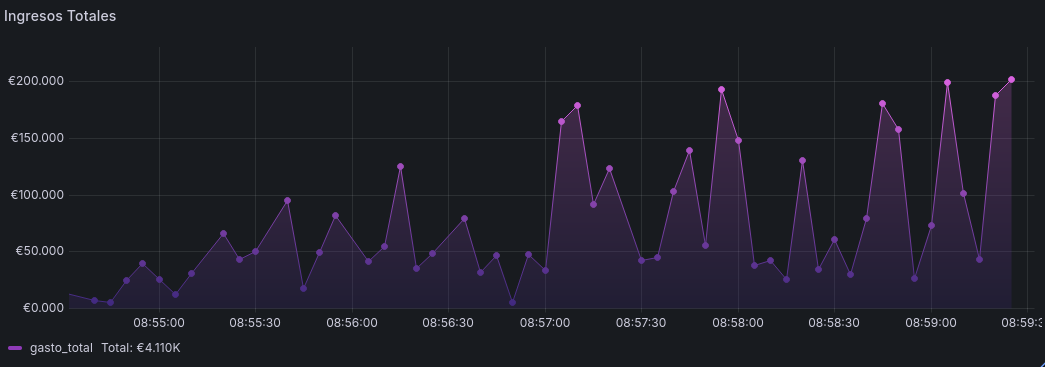
\includegraphics[width=1.0\linewidth]{ingT.png}
    \caption{Ingresos Totales}
    \label{fig:enter-label}
\end{figure}

\subsection*{Productos más vendidos}

Esta métrica también está dirigida a un ámbito comercial, ya que permite visualizar cuáles son los productos más vendidos en la web. Esta información puede ser útil para, por ejemplo, que el equipo comercial decida aumentar el stock de estos productos y ofrecer una mayor variedad en función de la demanda.

Para ello, dentro de Grafana se ha utilizado la siguiente sentencia SQL:

\begin{lstlisting}[language=SQL, style=SQL]
SELECT 
  id, nombre, total_pedidos
FROM (
  SELECT 
    p.id AS id,
    p.nombre AS nombre,
    COUNT(*) AS total_pedidos
  FROM 
    Carga_web.PedidoItem AS pe
  JOIN 
    Carga_web.Producto AS p ON p.id = pe.producto_id
  GROUP BY 
    p.id, p.nombre
  HAVING 
    COUNT(*) > 10

  UNION ALL

  SELECT 
    NULL AS id,
    'Sin resultados' AS nombre,
    NULL AS total_pedidos
  WHERE NOT EXISTS (
    SELECT 
      1
    FROM 
      Carga_web.PedidoItem AS pe
    JOIN 
      Carga_web.Producto AS p ON p.id = pe.producto_id
    GROUP BY 
      p.id, p.nombre
    HAVING 
      COUNT(*) > 10
  )
) AS datos
LIMIT 10;
\end{lstlisting}

Esta consulta permite obtener los productos con más de 10 pedidos y, en caso de que no existan, mostrar un mensaje indicando que no hay resultados. 

Para mostrar los datos en Grafana, se ha optado por una visualización de tipo *Table*, donde se puede observar el ID del producto, su nombre y el número total de pedidos en los que ha sido incluido. De esta forma, se puede construir un ranking con los 10 productos más vendidos y obtener una visualización clara y útil para la toma de decisiones.

\begin{figure}[!h]
    \centering
    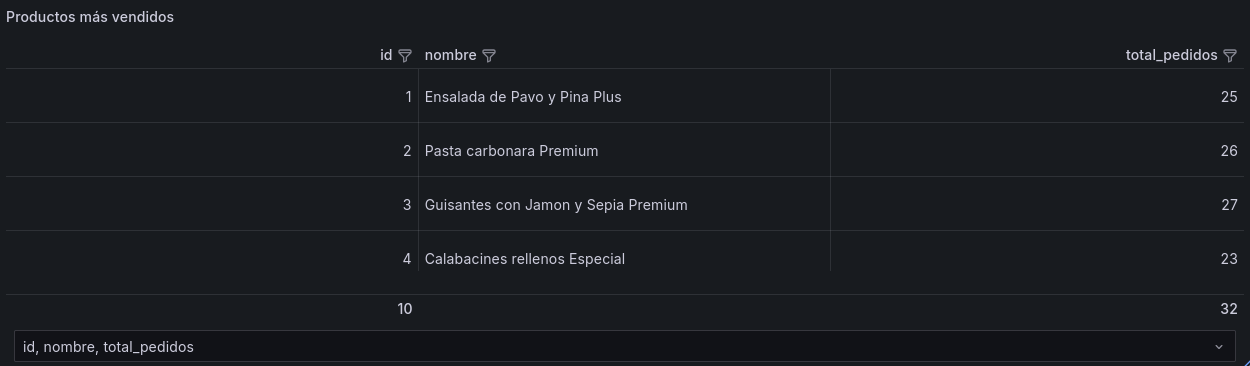
\includegraphics[width=1.0\linewidth]{productosV.png}
    \caption{Productos más vendidos}
    \label{fig:enter-label}
\end{figure}

\subsection*{Carritos de usuarios que tienen productos}

Esta métrica permite conocer cuántos carritos contienen productos y, por tanto, están listos o en preparación para realizar un pedido. El propósito principal es llevar un control sobre la carga de la base de datos, específicamente sobre la tabla `CarritoItem`. 

A partir de esta métrica también se podrían derivar otras, como por ejemplo, identificar carritos que contienen productos pero que no han finalizado el pedido tras un cierto tiempo, es decir, carritos potencialmente abandonados.

Para ello, dentro de Grafana se ha utilizado la siguiente sentencia SQL:

\begin{lstlisting}[language=SQL, style=SQL]
SELECT COUNT(DISTINCT ci.carrito_id) AS carritos_con_items
FROM Carga_web.CarritoItem ci
JOIN Carga_web.Carrito c ON c.id = ci.carrito_id;
\end{lstlisting}

Para mostrar los resultados en Grafana, se ha optado por una visualización de tipo *Gauge*, estableciendo un límite máximo de 150 carritos. Esta elección se debe a que, una vez que se realizan los pedidos, de tabla `CarritoItem` se eliminan los items del usurio que acaba de realizar el pedido, lo que hace que esta visualización varíe constantemente.

Además, esta métrica permite evaluar la carga que está soportando la tabla de carritos y analizar si los usuarios están avanzando en el proceso de compra o simplemente acumulando productos sin completar el pedido.

\begin{figure}[!h]
    \centering
    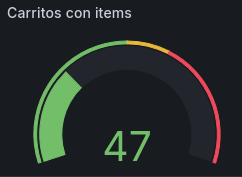
\includegraphics[width=0.3\linewidth]{carritoItems.png}
    \caption{Número de Carritos con Items}
    \label{fig:enter-label}
\end{figure}

\subsection*{Pedidos creados}

Esta métrica permite conocer cuántos pedidos se han realizado en cada unidad de tiempo, lo cual resulta útil para analizar el comportamiento de los usuarios en la web, detectar picos de actividad y evaluar el rendimiento del sistema. Además, también permite visualizar el número total de pedidos realizados en el intervalo seleccionado.

Para ello, dentro de Grafana se ha utilizado la siguiente sentencia SQL:

\begin{lstlisting}[language=SQL, style=SQL]
SELECT 
  (FLOOR(UNIX_TIMESTAMP(fecha) / 10) * 10) * 1000 AS time,
  COUNT(*) AS pedidos
FROM 
  Carga_web.Pedido
WHERE 
  $__timeFilter(fecha)
GROUP BY 
  time
ORDER BY 
  time;
\end{lstlisting}

Esta consulta agrupa los pedidos realizados en intervalos de 10 segundos, permitiendo así una visualización dinámica y detallada de la frecuencia de pedidos a lo largo del tiempo. La función `\_\_timeFilter(fecha)` es gestionada automáticamente por Grafana para adaptar el rango temporal a lo que el usuario seleccione en el panel.

Para mostrar los resultados en Grafana, se ha optado por una visualización de tipo *Time series*, que facilita el seguimiento temporal de los pedidos, ayudando a detectar patrones de comportamiento de los usuarios, así como a evaluar posibles cuellos de botella o momentos de alta demanda.
\begin{figure}[!h]
    \centering
    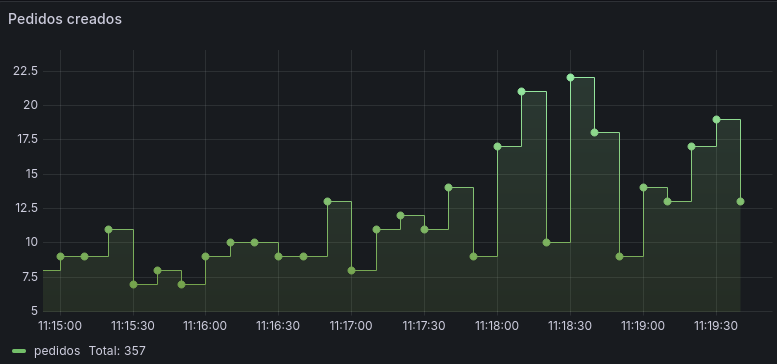
\includegraphics[width=0.7\linewidth]{pedCrea.png}
    \caption{Pedidos creados por unidad de tiempo y pedidos totales}
    \label{fig:enter-label}
\end{figure}

\section{Conclusiones Grafana}
Grafana ha contribuido de manera muy eficaz a la hora de recoger y visualizar los datos del sistema. Gracias a su fácil integración con bases de datos, hemos podido obtener los resultados necesarios y observar el comportamiento del sistema de forma clara y eficiente. Con una implementación sencilla y rápida, Grafana ha demostrado ser una herramienta robusta, permitiéndonos monitorizar el estado del sistema como si se tratara de un entorno real.

\chapter{Conclusiones y  Reparto de trabajo}

\section{Conclusiones Finales}

A lo largo de este proyecto se ha conseguido desarrollar una aplicación web en Flask, siguiendo una arquitectura Modelo-Vista-Controlador (MVC). Se han implementado las funcionalidades principales de una tienda online, como el registro y login de usuarios, la visualización de productos, la gestión de carritos y pedidos, así como un sistema de autenticación mediante tokens.

Por otro lado, se han realizado pruebas de carga sobre la página web y sus diferentes endpoints utilizando la herramienta Locust, desarrollada en Python. Para estas pruebas, se creó un script que simulaba diferentes usuarios realizando las distintas tareas posibles en nuestra web. Esto permitió exponer el sistema a distintas condiciones de carga. Tras las pruebas, se recogieron los resultados y se generaron métricas que ayudaron a identificar posibles cuellos de botella.

También se configuró Grafana para visualizar métricas del sistema, lo cual fue útil para observar el rendimiento en tiempo real y entender mejor el comportamiento de la aplicación bajo carga.

\subsubsection*{Problemas encontrados}
Durante el desarrollo de la web no surgieron demasiados problemas, aunque sí hubo algunos retos, especialmente al implementar los tokens de autenticación y al mostrar todos los pedidos de un usuario, ya que requería una lógica más elaborada. En cuanto a Locust, también hubo dificultades al principio, ya que no conocíamos bien la herramienta y los datos recogidos no eran fiables. Esto se debió a que no comprendíamos bien cómo se distribuían los usuarios ni cómo ejecutaban las tareas. Sin embargo, esto nos llevó a mejorar y escalar el código de manera más sólida.

\subsubsection*{En resumen}
Gracias a este proyecto hemos podido conocer herramientas de desarrollo backend como Flask, que ha resultado ser bastante intuitiva y fácil de usar. También diseñamos una base de datos relacional, lo cual ha reforzado nuestros conocimientos previos. Por otro lado, el uso de Locust nos ha enseñado lo sencillo que puede ser generar carga y evaluar el comportamiento de una web. Además, hemos conseguido aplicar los conocimientos teóricos de la asignatura a un caso práctico y real, lo que ha reforzado lo aprendido en clase. También hemos mejorado nuestras habilidades con Git y GitHub, trabajando de forma colaborativa.

\subsubsection*{Mejoras}
Como posibles mejoras futuras, se propone:
\begin{itemize}
    \item Mejorar el \textit{frontend} de la página web para ofrecer una mejor experiencia al usuario.
    \item Implementar medidas para balancear la carga y mejorar el rendimiento general.
    \item Extender los paneles de Grafana con más métricas de negocio.
\end{itemize}


\section{Reparto de trabajo}

\subsection{Trabajo personal}

\subsubsection*{Fernández Sánchez, Víctor}
\begin{itemize}
    \item \textbf{Página web}: Registro de usuarios, implementación del endpoint del carrito y del endpoint de productos.
    \item \textbf{Locust}: Tareas de checkout y de agregar productos al carrito.
\end{itemize}

\subsubsection*{Sánchez Maroto, Gonzalo}
\begin{itemize}
    \item \textbf{Página web}: Menú principal e implementación del endpoint de pedidos.
    \item \textbf{Locust}: Tareas de visualización de pedidos individuales, listados de pedidos y vaciado del carrito.
\end{itemize}

\subsubsection*{Sanz Santos, Diego}
\begin{itemize}
    \item \textbf{Página web}: Login de usuarios, implementación del endpoint del carrito y de pedidos, y generación del token de autenticación.
    \item \textbf{Locust}: Tareas de autenticación, cierre de sesión, visualización del menú, login y registro.
\end{itemize}

\subsubsection*{Verduras Cavada, Rubén}
\begin{itemize}
    \item \textbf{Página web}: Implementación del endpoint de pedidos y de productos, y desarrollo de funciones auxiliares.
    \item \textbf{Locust}: Tareas de visualización de productos y su modificación tanto total (PUT) como parcial (PATCH).
\end{itemize}

\subsection{Trabajo común}
\begin{itemize}
    \item \textbf{Página web}: Cada integrante se encargó de implementar distintos controladores, como se detalló anteriormente. Las clases y los \texttt{schemas} fueron repartidos entre todos, dividiéndose el trabajo de forma equitativa. El diseño del modelo de dominio y la estructura general de la aplicación se realizaron en conjunto.
    \item \textbf{Base de datos}: La estructura de las tablas y su creación se diseñaron en equipo, incluyendo los diagramas y los procedimientos almacenados.
    \item \textbf{Informe}: Su redacción se distribuyó de forma equitativa. Rubén, Víctor y Diego se centraron principalmente en las secciones relacionadas con Locust y la página web, mientras que Gonzalo trabajó más en la parte de la web y en la integración con Grafana.
\end{itemize}

\printbibliography
\end{document}
